% Options for packages loaded elsewhere
\PassOptionsToPackage{unicode}{hyperref}
\PassOptionsToPackage{hyphens}{url}
%
\documentclass[
]{article}
\usepackage{amsmath,amssymb}
\usepackage{lmodern}
\usepackage{iftex}
\ifPDFTeX
  \usepackage[T1]{fontenc}
  \usepackage[utf8]{inputenc}
  \usepackage{textcomp} % provide euro and other symbols
\else % if luatex or xetex
  \usepackage{unicode-math}
  \defaultfontfeatures{Scale=MatchLowercase}
  \defaultfontfeatures[\rmfamily]{Ligatures=TeX,Scale=1}
\fi
% Use upquote if available, for straight quotes in verbatim environments
\IfFileExists{upquote.sty}{\usepackage{upquote}}{}
\IfFileExists{microtype.sty}{% use microtype if available
  \usepackage[]{microtype}
  \UseMicrotypeSet[protrusion]{basicmath} % disable protrusion for tt fonts
}{}
\makeatletter
\@ifundefined{KOMAClassName}{% if non-KOMA class
  \IfFileExists{parskip.sty}{%
    \usepackage{parskip}
  }{% else
    \setlength{\parindent}{0pt}
    \setlength{\parskip}{6pt plus 2pt minus 1pt}}
}{% if KOMA class
  \KOMAoptions{parskip=half}}
\makeatother
\usepackage{xcolor}
\usepackage[margin=1in]{geometry}
\usepackage{color}
\usepackage{fancyvrb}
\newcommand{\VerbBar}{|}
\newcommand{\VERB}{\Verb[commandchars=\\\{\}]}
\DefineVerbatimEnvironment{Highlighting}{Verbatim}{commandchars=\\\{\}}
% Add ',fontsize=\small' for more characters per line
\usepackage{framed}
\definecolor{shadecolor}{RGB}{241,243,245}
\newenvironment{Shaded}{\begin{snugshade}}{\end{snugshade}}
\newcommand{\AlertTok}[1]{\textcolor[rgb]{0.68,0.00,0.00}{#1}}
\newcommand{\AnnotationTok}[1]{\textcolor[rgb]{0.37,0.37,0.37}{#1}}
\newcommand{\AttributeTok}[1]{\textcolor[rgb]{0.40,0.45,0.13}{#1}}
\newcommand{\BaseNTok}[1]{\textcolor[rgb]{0.68,0.00,0.00}{#1}}
\newcommand{\BuiltInTok}[1]{\textcolor[rgb]{0.00,0.46,0.62}{#1}}
\newcommand{\CharTok}[1]{\textcolor[rgb]{0.13,0.47,0.30}{#1}}
\newcommand{\CommentTok}[1]{\textcolor[rgb]{0.37,0.37,0.37}{#1}}
\newcommand{\CommentVarTok}[1]{\textcolor[rgb]{0.37,0.37,0.37}{\textit{#1}}}
\newcommand{\ConstantTok}[1]{\textcolor[rgb]{0.56,0.35,0.01}{#1}}
\newcommand{\ControlFlowTok}[1]{\textcolor[rgb]{0.00,0.46,0.62}{#1}}
\newcommand{\DataTypeTok}[1]{\textcolor[rgb]{0.68,0.00,0.00}{#1}}
\newcommand{\DecValTok}[1]{\textcolor[rgb]{0.68,0.00,0.00}{#1}}
\newcommand{\DocumentationTok}[1]{\textcolor[rgb]{0.37,0.37,0.37}{\textit{#1}}}
\newcommand{\ErrorTok}[1]{\textcolor[rgb]{0.68,0.00,0.00}{#1}}
\newcommand{\ExtensionTok}[1]{\textcolor[rgb]{0.00,0.46,0.62}{#1}}
\newcommand{\FloatTok}[1]{\textcolor[rgb]{0.68,0.00,0.00}{#1}}
\newcommand{\FunctionTok}[1]{\textcolor[rgb]{0.28,0.35,0.67}{#1}}
\newcommand{\ImportTok}[1]{\textcolor[rgb]{0.00,0.46,0.62}{#1}}
\newcommand{\InformationTok}[1]{\textcolor[rgb]{0.37,0.37,0.37}{#1}}
\newcommand{\KeywordTok}[1]{\textcolor[rgb]{0.00,0.46,0.62}{#1}}
\newcommand{\NormalTok}[1]{\textcolor[rgb]{0.00,0.46,0.62}{#1}}
\newcommand{\OperatorTok}[1]{\textcolor[rgb]{0.37,0.37,0.37}{#1}}
\newcommand{\OtherTok}[1]{\textcolor[rgb]{0.00,0.46,0.62}{#1}}
\newcommand{\PreprocessorTok}[1]{\textcolor[rgb]{0.68,0.00,0.00}{#1}}
\newcommand{\RegionMarkerTok}[1]{\textcolor[rgb]{0.00,0.46,0.62}{#1}}
\newcommand{\SpecialCharTok}[1]{\textcolor[rgb]{0.37,0.37,0.37}{#1}}
\newcommand{\SpecialStringTok}[1]{\textcolor[rgb]{0.13,0.47,0.30}{#1}}
\newcommand{\StringTok}[1]{\textcolor[rgb]{0.13,0.47,0.30}{#1}}
\newcommand{\VariableTok}[1]{\textcolor[rgb]{0.07,0.07,0.07}{#1}}
\newcommand{\VerbatimStringTok}[1]{\textcolor[rgb]{0.13,0.47,0.30}{#1}}
\newcommand{\WarningTok}[1]{\textcolor[rgb]{0.37,0.37,0.37}{\textit{#1}}}
\usepackage{longtable,booktabs,array}
\usepackage{multirow}
\usepackage{calc} % for calculating minipage widths
% Correct order of tables after \paragraph or \subparagraph
\usepackage{etoolbox}
\makeatletter
\patchcmd\longtable{\par}{\if@noskipsec\mbox{}\fi\par}{}{}
\makeatother
% Allow footnotes in longtable head/foot
\IfFileExists{footnotehyper.sty}{\usepackage{footnotehyper}}{\usepackage{footnote}}
\makesavenoteenv{longtable}
\usepackage{graphicx}
\makeatletter
\def\maxwidth{\ifdim\Gin@nat@width>\linewidth\linewidth\else\Gin@nat@width\fi}
\def\maxheight{\ifdim\Gin@nat@height>\textheight\textheight\else\Gin@nat@height\fi}
\makeatother
% Scale images if necessary, so that they will not overflow the page
% margins by default, and it is still possible to overwrite the defaults
% using explicit options in \includegraphics[width, height, ...]{}
\setkeys{Gin}{width=\maxwidth,height=\maxheight,keepaspectratio}
% Set default figure placement to htbp
\makeatletter
\def\fps@figure{htbp}
\makeatother
\setlength{\emergencystretch}{3em} % prevent overfull lines
\providecommand{\tightlist}{%
  \setlength{\itemsep}{0pt}\setlength{\parskip}{0pt}}
\setcounter{secnumdepth}{5}
\usepackage{newunicodechar}
\usepackage{amsmath}

\providecommand{\xelatexemojipath}[1]{images/#1}

\newcommand{\xelatexemoji}[1]{%
    \raisebox{-0.15em}{%
      \includegraphics[height=1em]{\xelatexemojipath{#1}}%
    }%
}

\newunicodechar{©}{\xelatexemoji{00a9}}
\newunicodechar{®}{\xelatexemoji{00ae}}
\newunicodechar{ࡦ}{\xelatexemoji{866}}
\newunicodechar{ᙕ}{\xelatexemoji{1655}}
\newunicodechar{‼}{\xelatexemoji{203c}}
\newunicodechar{⁉}{\xelatexemoji{2049}}
\newunicodechar{™}{\xelatexemoji{2122}}
\newunicodechar{ℹ}{\xelatexemoji{2139}}
\newunicodechar{↔}{\xelatexemoji{2194}}
\newunicodechar{↕}{\xelatexemoji{2195}}
\newunicodechar{↖}{\xelatexemoji{2196}}
\newunicodechar{↗}{\xelatexemoji{2197}}
\newunicodechar{↘}{\xelatexemoji{2198}}
\newunicodechar{↙}{\xelatexemoji{2199}}
\newunicodechar{↩}{\xelatexemoji{21a9}}
\newunicodechar{↪}{\xelatexemoji{21aa}}
\newunicodechar{⌚}{\xelatexemoji{231a}}
\newunicodechar{⌛}{\xelatexemoji{231b}}
\newunicodechar{⌨}{\xelatexemoji{2328}}
\newunicodechar{⏩}{\xelatexemoji{23e9}}
\newunicodechar{⏪}{\xelatexemoji{23ea}}
\newunicodechar{⏫}{\xelatexemoji{23eb}}
\newunicodechar{⏬}{\xelatexemoji{23ec}}
\newunicodechar{⏭}{\xelatexemoji{23ed}}
\newunicodechar{⏮}{\xelatexemoji{23ee}}
\newunicodechar{⏯}{\xelatexemoji{23ef}}
\newunicodechar{⏰}{\xelatexemoji{23f0}}
\newunicodechar{⏱}{\xelatexemoji{23f1}}
\newunicodechar{⏲}{\xelatexemoji{23f2}}
\newunicodechar{⏳}{\xelatexemoji{23f3}}
\newunicodechar{⏸}{\xelatexemoji{23f8}}
\newunicodechar{⏹}{\xelatexemoji{23f9}}
\newunicodechar{⏺}{\xelatexemoji{23fa}}
\newunicodechar{Ⓜ}{\xelatexemoji{24c2}}
\newunicodechar{▪}{\xelatexemoji{25aa}}
\newunicodechar{▫}{\xelatexemoji{25ab}}
\newunicodechar{▶}{\xelatexemoji{25b6}}
\newunicodechar{◀}{\xelatexemoji{25c0}}
\newunicodechar{◻}{\xelatexemoji{25fb}}
\newunicodechar{◼}{\xelatexemoji{25fc}}
\newunicodechar{◽}{\xelatexemoji{25fd}}
\newunicodechar{◾}{\xelatexemoji{25fe}}
\newunicodechar{☀}{\xelatexemoji{2600}}
\newunicodechar{☁}{\xelatexemoji{2601}}
\newunicodechar{☂}{\xelatexemoji{2602}}
\newunicodechar{☃}{\xelatexemoji{2603}}
\newunicodechar{☄}{\xelatexemoji{2604}}
\newunicodechar{☎}{\xelatexemoji{260e}}
\newunicodechar{☑}{\xelatexemoji{2611}}
\newunicodechar{☔}{\xelatexemoji{2614}}
\newunicodechar{☕}{\xelatexemoji{2615}}
\newunicodechar{☘}{\xelatexemoji{2618}}
\newunicodechar{☝}{\xelatexemoji{261d}}
\newunicodechar{☠}{\xelatexemoji{2620}}
\newunicodechar{☢}{\xelatexemoji{2622}}
\newunicodechar{☣}{\xelatexemoji{2623}}
\newunicodechar{☦}{\xelatexemoji{2626}}
\newunicodechar{☪}{\xelatexemoji{262a}}
\newunicodechar{☮}{\xelatexemoji{262e}}
\newunicodechar{☯}{\xelatexemoji{262f}}
\newunicodechar{☸}{\xelatexemoji{2638}}
\newunicodechar{☹}{\xelatexemoji{2639}}
\newunicodechar{☺}{\xelatexemoji{263a}}
\newunicodechar{♈}{\xelatexemoji{2648}}
\newunicodechar{♉}{\xelatexemoji{2649}}
\newunicodechar{♊}{\xelatexemoji{264a}}
\newunicodechar{♋}{\xelatexemoji{264b}}
\newunicodechar{♌}{\xelatexemoji{264c}}
\newunicodechar{♍}{\xelatexemoji{264d}}
\newunicodechar{♎}{\xelatexemoji{264e}}
\newunicodechar{♏}{\xelatexemoji{264f}}
\newunicodechar{♐}{\xelatexemoji{2650}}
\newunicodechar{♑}{\xelatexemoji{2651}}
\newunicodechar{♒}{\xelatexemoji{2652}}
\newunicodechar{♓}{\xelatexemoji{2653}}
\newunicodechar{♠}{\xelatexemoji{2660}}
\newunicodechar{♣}{\xelatexemoji{2663}}
\newunicodechar{♥}{\xelatexemoji{2665}}
\newunicodechar{♦}{\xelatexemoji{2666}}
\newunicodechar{♨}{\xelatexemoji{2668}}
\newunicodechar{♻}{\xelatexemoji{267b}}
\newunicodechar{♿}{\xelatexemoji{267f}}
\newunicodechar{⚒}{\xelatexemoji{2692}}
\newunicodechar{⚓}{\xelatexemoji{2693}}
\newunicodechar{⚔}{\xelatexemoji{2694}}
\newunicodechar{⚖}{\xelatexemoji{2696}}
\newunicodechar{⚗}{\xelatexemoji{2697}}
\newunicodechar{⚙}{\xelatexemoji{2699}}
\newunicodechar{⚛}{\xelatexemoji{269b}}
\newunicodechar{⚜}{\xelatexemoji{269c}}
\newunicodechar{⚠}{\xelatexemoji{26a0}}
\newunicodechar{⚡}{\xelatexemoji{26a1}}
\newunicodechar{⚪}{\xelatexemoji{26aa}}
\newunicodechar{⚫}{\xelatexemoji{26ab}}
\newunicodechar{⚰}{\xelatexemoji{26b0}}
\newunicodechar{⚱}{\xelatexemoji{26b1}}
\newunicodechar{⚽}{\xelatexemoji{26bd}}
\newunicodechar{⚾}{\xelatexemoji{26be}}
\newunicodechar{⛄}{\xelatexemoji{26c4}}
\newunicodechar{⛅}{\xelatexemoji{26c5}}
\newunicodechar{⛈}{\xelatexemoji{26c8}}
\newunicodechar{⛎}{\xelatexemoji{26ce}}
\newunicodechar{⛏}{\xelatexemoji{26cf}}
\newunicodechar{⛑}{\xelatexemoji{26d1}}
\newunicodechar{⛓}{\xelatexemoji{26d3}}
\newunicodechar{⛔}{\xelatexemoji{26d4}}
\newunicodechar{⛩}{\xelatexemoji{26e9}}
\newunicodechar{⛪}{\xelatexemoji{26ea}}
\newunicodechar{⛰}{\xelatexemoji{26f0}}
\newunicodechar{⛱}{\xelatexemoji{26f1}}
\newunicodechar{⛲}{\xelatexemoji{26f2}}
\newunicodechar{⛳}{\xelatexemoji{26f3}}
\newunicodechar{⛴}{\xelatexemoji{26f4}}
\newunicodechar{⛵}{\xelatexemoji{26f5}}
\newunicodechar{⛷}{\xelatexemoji{26f7}}
\newunicodechar{⛸}{\xelatexemoji{26f8}}
\newunicodechar{⛹}{\xelatexemoji{26f9}}
\newunicodechar{⛺}{\xelatexemoji{26fa}}
\newunicodechar{⛽}{\xelatexemoji{26fd}}
\newunicodechar{✂}{\xelatexemoji{2702}}
\newunicodechar{✅}{\xelatexemoji{2705}}
\newunicodechar{✈}{\xelatexemoji{2708}}
\newunicodechar{✉}{\xelatexemoji{2709}}
\newunicodechar{✊}{\xelatexemoji{270a}}
\newunicodechar{✋}{\xelatexemoji{270b}}
\newunicodechar{✌}{\xelatexemoji{270c}}
\newunicodechar{✍}{\xelatexemoji{270d}}
\newunicodechar{✏}{\xelatexemoji{270f}}
\newunicodechar{✒}{\xelatexemoji{2712}}
\newunicodechar{✔}{\xelatexemoji{2714}}
\newunicodechar{✖}{\xelatexemoji{2716}}
\newunicodechar{✝}{\xelatexemoji{271d}}
\newunicodechar{✡}{\xelatexemoji{2721}}
\newunicodechar{✨}{\xelatexemoji{2728}}
\newunicodechar{✳}{\xelatexemoji{2733}}
\newunicodechar{✴}{\xelatexemoji{2734}}
\newunicodechar{❄}{\xelatexemoji{2744}}
\newunicodechar{❇}{\xelatexemoji{2747}}
\newunicodechar{❌}{\xelatexemoji{274c}}
\newunicodechar{❎}{\xelatexemoji{274e}}
\newunicodechar{❓}{\xelatexemoji{2753}}
\newunicodechar{❔}{\xelatexemoji{2754}}
\newunicodechar{❕}{\xelatexemoji{2755}}
\newunicodechar{❗}{\xelatexemoji{2757}}
\newunicodechar{❣}{\xelatexemoji{2763}}
\newunicodechar{❤}{\xelatexemoji{2764}}
\newunicodechar{➕}{\xelatexemoji{2795}}
\newunicodechar{➖}{\xelatexemoji{2796}}
\newunicodechar{➗}{\xelatexemoji{2797}}
\newunicodechar{➡}{\xelatexemoji{27a1}}
\newunicodechar{➰}{\xelatexemoji{27b0}}
\newunicodechar{➿}{\xelatexemoji{27bf}}
\newunicodechar{⤴}{\xelatexemoji{2934}}
\newunicodechar{⤵}{\xelatexemoji{2935}}
\newunicodechar{⬅}{\xelatexemoji{2b05}}
\newunicodechar{⬆}{\xelatexemoji{2b06}}
\newunicodechar{⬇}{\xelatexemoji{2b07}}
\newunicodechar{⬛}{\xelatexemoji{2b1b}}
\newunicodechar{⬜}{\xelatexemoji{2b1c}}
\newunicodechar{⭐}{\xelatexemoji{2b50}}
\newunicodechar{⭕}{\xelatexemoji{2b55}}
\newunicodechar{〰}{\xelatexemoji{3030}}
\newunicodechar{〽}{\xelatexemoji{303d}}
\newunicodechar{㊗}{\xelatexemoji{3297}}
\newunicodechar{㊙}{\xelatexemoji{3299}}
\newunicodechar{🀄}{\xelatexemoji{1f004}}
\newunicodechar{🃏}{\xelatexemoji{1f0cf}}
\newunicodechar{🅰}{\xelatexemoji{1f170}}
\newunicodechar{🅱}{\xelatexemoji{1f171}}
\newunicodechar{🅾}{\xelatexemoji{1f17e}}
\newunicodechar{🅿}{\xelatexemoji{1f17f}}
\newunicodechar{🆎}{\xelatexemoji{1f18e}}
\newunicodechar{🆑}{\xelatexemoji{1f191}}
\newunicodechar{🆒}{\xelatexemoji{1f192}}
\newunicodechar{🆓}{\xelatexemoji{1f193}}
\newunicodechar{🆔}{\xelatexemoji{1f194}}
\newunicodechar{🆕}{\xelatexemoji{1f195}}
\newunicodechar{🆖}{\xelatexemoji{1f196}}
\newunicodechar{🆗}{\xelatexemoji{1f197}}
\newunicodechar{🆘}{\xelatexemoji{1f198}}
\newunicodechar{🆙}{\xelatexemoji{1f199}}
\newunicodechar{🆚}{\xelatexemoji{1f19a}}
\newunicodechar{🈁}{\xelatexemoji{1f201}}
\newunicodechar{🈂}{\xelatexemoji{1f202}}
\newunicodechar{🈚}{\xelatexemoji{1f21a}}
\newunicodechar{🈯}{\xelatexemoji{1f22f}}
\newunicodechar{🈲}{\xelatexemoji{1f232}}
\newunicodechar{🈳}{\xelatexemoji{1f233}}
\newunicodechar{🈴}{\xelatexemoji{1f234}}
\newunicodechar{🈵}{\xelatexemoji{1f235}}
\newunicodechar{🈶}{\xelatexemoji{1f236}}
\newunicodechar{🈷}{\xelatexemoji{1f237}}
\newunicodechar{🈸}{\xelatexemoji{1f238}}
\newunicodechar{🈹}{\xelatexemoji{1f239}}
\newunicodechar{🈺}{\xelatexemoji{1f23a}}
\newunicodechar{🉐}{\xelatexemoji{1f250}}
\newunicodechar{🉑}{\xelatexemoji{1f251}}
\newunicodechar{🌀}{\xelatexemoji{1f300}}
\newunicodechar{🌁}{\xelatexemoji{1f301}}
\newunicodechar{🌂}{\xelatexemoji{1f302}}
\newunicodechar{🌃}{\xelatexemoji{1f303}}
\newunicodechar{🌄}{\xelatexemoji{1f304}}
\newunicodechar{🌅}{\xelatexemoji{1f305}}
\newunicodechar{🌆}{\xelatexemoji{1f306}}
\newunicodechar{🌇}{\xelatexemoji{1f307}}
\newunicodechar{🌈}{\xelatexemoji{1f308}}
\newunicodechar{🌉}{\xelatexemoji{1f309}}
\newunicodechar{🌊}{\xelatexemoji{1f30a}}
\newunicodechar{🌋}{\xelatexemoji{1f30b}}
\newunicodechar{🌌}{\xelatexemoji{1f30c}}
\newunicodechar{🌍}{\xelatexemoji{1f30d}}
\newunicodechar{🌎}{\xelatexemoji{1f30e}}
\newunicodechar{🌏}{\xelatexemoji{1f30f}}
\newunicodechar{🌐}{\xelatexemoji{1f310}}
\newunicodechar{🌑}{\xelatexemoji{1f311}}
\newunicodechar{🌒}{\xelatexemoji{1f312}}
\newunicodechar{🌓}{\xelatexemoji{1f313}}
\newunicodechar{🌔}{\xelatexemoji{1f314}}
\newunicodechar{🌕}{\xelatexemoji{1f315}}
\newunicodechar{🌖}{\xelatexemoji{1f316}}
\newunicodechar{🌗}{\xelatexemoji{1f317}}
\newunicodechar{🌘}{\xelatexemoji{1f318}}
\newunicodechar{🌙}{\xelatexemoji{1f319}}
\newunicodechar{🌚}{\xelatexemoji{1f31a}}
\newunicodechar{🌛}{\xelatexemoji{1f31b}}
\newunicodechar{🌜}{\xelatexemoji{1f31c}}
\newunicodechar{🌝}{\xelatexemoji{1f31d}}
\newunicodechar{🌞}{\xelatexemoji{1f31e}}
\newunicodechar{🌟}{\xelatexemoji{1f31f}}
\newunicodechar{🌠}{\xelatexemoji{1f320}}
\newunicodechar{🌡}{\xelatexemoji{1f321}}
\newunicodechar{🌤}{\xelatexemoji{1f324}}
\newunicodechar{🌥}{\xelatexemoji{1f325}}
\newunicodechar{🌦}{\xelatexemoji{1f326}}
\newunicodechar{🌧}{\xelatexemoji{1f327}}
\newunicodechar{🌨}{\xelatexemoji{1f328}}
\newunicodechar{🌩}{\xelatexemoji{1f329}}
\newunicodechar{🌪}{\xelatexemoji{1f32a}}
\newunicodechar{🌫}{\xelatexemoji{1f32b}}
\newunicodechar{🌬}{\xelatexemoji{1f32c}}
\newunicodechar{🌭}{\xelatexemoji{1f32d}}
\newunicodechar{🌮}{\xelatexemoji{1f32e}}
\newunicodechar{🌯}{\xelatexemoji{1f32f}}
\newunicodechar{🌰}{\xelatexemoji{1f330}}
\newunicodechar{🌱}{\xelatexemoji{1f331}}
\newunicodechar{🌲}{\xelatexemoji{1f332}}
\newunicodechar{🌳}{\xelatexemoji{1f333}}
\newunicodechar{🌴}{\xelatexemoji{1f334}}
\newunicodechar{🌵}{\xelatexemoji{1f335}}
\newunicodechar{🌶}{\xelatexemoji{1f336}}
\newunicodechar{🌷}{\xelatexemoji{1f337}}
\newunicodechar{🌸}{\xelatexemoji{1f338}}
\newunicodechar{🌹}{\xelatexemoji{1f339}}
\newunicodechar{🌺}{\xelatexemoji{1f33a}}
\newunicodechar{🌻}{\xelatexemoji{1f33b}}
\newunicodechar{🌼}{\xelatexemoji{1f33c}}
\newunicodechar{🌽}{\xelatexemoji{1f33d}}
\newunicodechar{🌾}{\xelatexemoji{1f33e}}
\newunicodechar{🌿}{\xelatexemoji{1f33f}}
\newunicodechar{🍀}{\xelatexemoji{1f340}}
\newunicodechar{🍁}{\xelatexemoji{1f341}}
\newunicodechar{🍂}{\xelatexemoji{1f342}}
\newunicodechar{🍃}{\xelatexemoji{1f343}}
\newunicodechar{🍄}{\xelatexemoji{1f344}}
\newunicodechar{🍅}{\xelatexemoji{1f345}}
\newunicodechar{🍆}{\xelatexemoji{1f346}}
\newunicodechar{🍇}{\xelatexemoji{1f347}}
\newunicodechar{🍈}{\xelatexemoji{1f348}}
\newunicodechar{🍉}{\xelatexemoji{1f349}}
\newunicodechar{🍊}{\xelatexemoji{1f34a}}
\newunicodechar{🍋}{\xelatexemoji{1f34b}}
\newunicodechar{🍌}{\xelatexemoji{1f34c}}
\newunicodechar{🍍}{\xelatexemoji{1f34d}}
\newunicodechar{🍎}{\xelatexemoji{1f34e}}
\newunicodechar{🍏}{\xelatexemoji{1f34f}}
\newunicodechar{🍐}{\xelatexemoji{1f350}}
\newunicodechar{🍑}{\xelatexemoji{1f351}}
\newunicodechar{🍒}{\xelatexemoji{1f352}}
\newunicodechar{🍓}{\xelatexemoji{1f353}}
\newunicodechar{🍔}{\xelatexemoji{1f354}}
\newunicodechar{🍕}{\xelatexemoji{1f355}}
\newunicodechar{🍖}{\xelatexemoji{1f356}}
\newunicodechar{🍗}{\xelatexemoji{1f357}}
\newunicodechar{🍘}{\xelatexemoji{1f358}}
\newunicodechar{🍙}{\xelatexemoji{1f359}}
\newunicodechar{🍚}{\xelatexemoji{1f35a}}
\newunicodechar{🍛}{\xelatexemoji{1f35b}}
\newunicodechar{🍜}{\xelatexemoji{1f35c}}
\newunicodechar{🍝}{\xelatexemoji{1f35d}}
\newunicodechar{🍞}{\xelatexemoji{1f35e}}
\newunicodechar{🍟}{\xelatexemoji{1f35f}}
\newunicodechar{🍠}{\xelatexemoji{1f360}}
\newunicodechar{🍡}{\xelatexemoji{1f361}}
\newunicodechar{🍢}{\xelatexemoji{1f362}}
\newunicodechar{🍣}{\xelatexemoji{1f363}}
\newunicodechar{🍤}{\xelatexemoji{1f364}}
\newunicodechar{🍥}{\xelatexemoji{1f365}}
\newunicodechar{🍦}{\xelatexemoji{1f366}}
\newunicodechar{🍧}{\xelatexemoji{1f367}}
\newunicodechar{🍨}{\xelatexemoji{1f368}}
\newunicodechar{🍩}{\xelatexemoji{1f369}}
\newunicodechar{🍪}{\xelatexemoji{1f36a}}
\newunicodechar{🍫}{\xelatexemoji{1f36b}}
\newunicodechar{🍬}{\xelatexemoji{1f36c}}
\newunicodechar{🍭}{\xelatexemoji{1f36d}}
\newunicodechar{🍮}{\xelatexemoji{1f36e}}
\newunicodechar{🍯}{\xelatexemoji{1f36f}}
\newunicodechar{🍰}{\xelatexemoji{1f370}}
\newunicodechar{🍱}{\xelatexemoji{1f371}}
\newunicodechar{🍲}{\xelatexemoji{1f372}}
\newunicodechar{🍳}{\xelatexemoji{1f373}}
\newunicodechar{🍴}{\xelatexemoji{1f374}}
\newunicodechar{🍵}{\xelatexemoji{1f375}}
\newunicodechar{🍶}{\xelatexemoji{1f376}}
\newunicodechar{🍷}{\xelatexemoji{1f377}}
\newunicodechar{🍸}{\xelatexemoji{1f378}}
\newunicodechar{🍹}{\xelatexemoji{1f379}}
\newunicodechar{🍺}{\xelatexemoji{1f37a}}
\newunicodechar{🍻}{\xelatexemoji{1f37b}}
\newunicodechar{🍼}{\xelatexemoji{1f37c}}
\newunicodechar{🍽}{\xelatexemoji{1f37d}}
\newunicodechar{🍾}{\xelatexemoji{1f37e}}
\newunicodechar{🍿}{\xelatexemoji{1f37f}}
\newunicodechar{🎀}{\xelatexemoji{1f380}}
\newunicodechar{🎁}{\xelatexemoji{1f381}}
\newunicodechar{🎂}{\xelatexemoji{1f382}}
\newunicodechar{🎃}{\xelatexemoji{1f383}}
\newunicodechar{🎄}{\xelatexemoji{1f384}}
\newunicodechar{🎅}{\xelatexemoji{1f385}}
\newunicodechar{🎆}{\xelatexemoji{1f386}}
\newunicodechar{🎇}{\xelatexemoji{1f387}}
\newunicodechar{🎈}{\xelatexemoji{1f388}}
\newunicodechar{🎉}{\xelatexemoji{1f389}}
\newunicodechar{🎊}{\xelatexemoji{1f38a}}
\newunicodechar{🎋}{\xelatexemoji{1f38b}}
\newunicodechar{🎌}{\xelatexemoji{1f38c}}
\newunicodechar{🎍}{\xelatexemoji{1f38d}}
\newunicodechar{🎎}{\xelatexemoji{1f38e}}
\newunicodechar{🎏}{\xelatexemoji{1f38f}}
\newunicodechar{🎐}{\xelatexemoji{1f390}}
\newunicodechar{🎑}{\xelatexemoji{1f391}}
\newunicodechar{🎒}{\xelatexemoji{1f392}}
\newunicodechar{🎓}{\xelatexemoji{1f393}}
\newunicodechar{🎖}{\xelatexemoji{1f396}}
\newunicodechar{🎗}{\xelatexemoji{1f397}}
\newunicodechar{🎙}{\xelatexemoji{1f399}}
\newunicodechar{🎚}{\xelatexemoji{1f39a}}
\newunicodechar{🎛}{\xelatexemoji{1f39b}}
\newunicodechar{🎞}{\xelatexemoji{1f39e}}
\newunicodechar{🎟}{\xelatexemoji{1f39f}}
\newunicodechar{🎠}{\xelatexemoji{1f3a0}}
\newunicodechar{🎡}{\xelatexemoji{1f3a1}}
\newunicodechar{🎢}{\xelatexemoji{1f3a2}}
\newunicodechar{🎣}{\xelatexemoji{1f3a3}}
\newunicodechar{🎤}{\xelatexemoji{1f3a4}}
\newunicodechar{🎥}{\xelatexemoji{1f3a5}}
\newunicodechar{🎦}{\xelatexemoji{1f3a6}}
\newunicodechar{🎧}{\xelatexemoji{1f3a7}}
\newunicodechar{🎨}{\xelatexemoji{1f3a8}}
\newunicodechar{🎩}{\xelatexemoji{1f3a9}}
\newunicodechar{🎪}{\xelatexemoji{1f3aa}}
\newunicodechar{🎫}{\xelatexemoji{1f3ab}}
\newunicodechar{🎬}{\xelatexemoji{1f3ac}}
\newunicodechar{🎭}{\xelatexemoji{1f3ad}}
\newunicodechar{🎮}{\xelatexemoji{1f3ae}}
\newunicodechar{🎯}{\xelatexemoji{1f3af}}
\newunicodechar{🎰}{\xelatexemoji{1f3b0}}
\newunicodechar{🎱}{\xelatexemoji{1f3b1}}
\newunicodechar{🎲}{\xelatexemoji{1f3b2}}
\newunicodechar{🎳}{\xelatexemoji{1f3b3}}
\newunicodechar{🎴}{\xelatexemoji{1f3b4}}
\newunicodechar{🎵}{\xelatexemoji{1f3b5}}
\newunicodechar{🎶}{\xelatexemoji{1f3b6}}
\newunicodechar{🎷}{\xelatexemoji{1f3b7}}
\newunicodechar{🎸}{\xelatexemoji{1f3b8}}
\newunicodechar{🎹}{\xelatexemoji{1f3b9}}
\newunicodechar{🎺}{\xelatexemoji{1f3ba}}
\newunicodechar{🎻}{\xelatexemoji{1f3bb}}
\newunicodechar{🎼}{\xelatexemoji{1f3bc}}
\newunicodechar{🎽}{\xelatexemoji{1f3bd}}
\newunicodechar{🎾}{\xelatexemoji{1f3be}}
\newunicodechar{🎿}{\xelatexemoji{1f3bf}}
\newunicodechar{🏀}{\xelatexemoji{1f3c0}}
\newunicodechar{🏁}{\xelatexemoji{1f3c1}}
\newunicodechar{🏂}{\xelatexemoji{1f3c2}}
\newunicodechar{🏃}{\xelatexemoji{1f3c3}}
\newunicodechar{🏄}{\xelatexemoji{1f3c4}}
\newunicodechar{🏅}{\xelatexemoji{1f3c5}}
\newunicodechar{🏆}{\xelatexemoji{1f3c6}}
\newunicodechar{🏇}{\xelatexemoji{1f3c7}}
\newunicodechar{🏈}{\xelatexemoji{1f3c8}}
\newunicodechar{🏉}{\xelatexemoji{1f3c9}}
\newunicodechar{🏊}{\xelatexemoji{1f3ca}}
\newunicodechar{🏋}{\xelatexemoji{1f3cb}}
\newunicodechar{🏌}{\xelatexemoji{1f3cc}}
\newunicodechar{🏍}{\xelatexemoji{1f3cd}}
\newunicodechar{🏎}{\xelatexemoji{1f3ce}}
\newunicodechar{🏏}{\xelatexemoji{1f3cf}}
\newunicodechar{🏐}{\xelatexemoji{1f3d0}}
\newunicodechar{🏑}{\xelatexemoji{1f3d1}}
\newunicodechar{🏒}{\xelatexemoji{1f3d2}}
\newunicodechar{🏓}{\xelatexemoji{1f3d3}}
\newunicodechar{🏔}{\xelatexemoji{1f3d4}}
\newunicodechar{🏕}{\xelatexemoji{1f3d5}}
\newunicodechar{🏖}{\xelatexemoji{1f3d6}}
\newunicodechar{🏗}{\xelatexemoji{1f3d7}}
\newunicodechar{🏘}{\xelatexemoji{1f3d8}}
\newunicodechar{🏙}{\xelatexemoji{1f3d9}}
\newunicodechar{🏚}{\xelatexemoji{1f3da}}
\newunicodechar{🏛}{\xelatexemoji{1f3db}}
\newunicodechar{🏜}{\xelatexemoji{1f3dc}}
\newunicodechar{🏝}{\xelatexemoji{1f3dd}}
\newunicodechar{🏞}{\xelatexemoji{1f3de}}
\newunicodechar{🏟}{\xelatexemoji{1f3df}}
\newunicodechar{🏠}{\xelatexemoji{1f3e0}}
\newunicodechar{🏡}{\xelatexemoji{1f3e1}}
\newunicodechar{🏢}{\xelatexemoji{1f3e2}}
\newunicodechar{🏣}{\xelatexemoji{1f3e3}}
\newunicodechar{🏤}{\xelatexemoji{1f3e4}}
\newunicodechar{🏥}{\xelatexemoji{1f3e5}}
\newunicodechar{🏦}{\xelatexemoji{1f3e6}}
\newunicodechar{🏧}{\xelatexemoji{1f3e7}}
\newunicodechar{🏨}{\xelatexemoji{1f3e8}}
\newunicodechar{🏩}{\xelatexemoji{1f3e9}}
\newunicodechar{🏪}{\xelatexemoji{1f3ea}}
\newunicodechar{🏫}{\xelatexemoji{1f3eb}}
\newunicodechar{🏬}{\xelatexemoji{1f3ec}}
\newunicodechar{🏭}{\xelatexemoji{1f3ed}}
\newunicodechar{🏮}{\xelatexemoji{1f3ee}}
\newunicodechar{🏯}{\xelatexemoji{1f3ef}}
\newunicodechar{🏰}{\xelatexemoji{1f3f0}}
\newunicodechar{🏳}{\xelatexemoji{1f3f3}}
\newunicodechar{🏴}{\xelatexemoji{1f3f4}}
\newunicodechar{🏵}{\xelatexemoji{1f3f5}}
\newunicodechar{🏷}{\xelatexemoji{1f3f7}}
\newunicodechar{🏸}{\xelatexemoji{1f3f8}}
\newunicodechar{🏹}{\xelatexemoji{1f3f9}}
\newunicodechar{🏺}{\xelatexemoji{1f3fa}}
\newunicodechar{🏻}{\xelatexemoji{1f3fb}}
\newunicodechar{🏼}{\xelatexemoji{1f3fc}}
\newunicodechar{🏽}{\xelatexemoji{1f3fd}}
\newunicodechar{🏾}{\xelatexemoji{1f3fe}}
\newunicodechar{🏿}{\xelatexemoji{1f3ff}}
\newunicodechar{🐀}{\xelatexemoji{1f400}}
\newunicodechar{🐁}{\xelatexemoji{1f401}}
\newunicodechar{🐂}{\xelatexemoji{1f402}}
\newunicodechar{🐃}{\xelatexemoji{1f403}}
\newunicodechar{🐄}{\xelatexemoji{1f404}}
\newunicodechar{🐅}{\xelatexemoji{1f405}}
\newunicodechar{🐆}{\xelatexemoji{1f406}}
\newunicodechar{🐇}{\xelatexemoji{1f407}}
\newunicodechar{🐈}{\xelatexemoji{1f408}}
\newunicodechar{🐉}{\xelatexemoji{1f409}}
\newunicodechar{🐊}{\xelatexemoji{1f40a}}
\newunicodechar{🐋}{\xelatexemoji{1f40b}}
\newunicodechar{🐌}{\xelatexemoji{1f40c}}
\newunicodechar{🐍}{\xelatexemoji{1f40d}}
\newunicodechar{🐎}{\xelatexemoji{1f40e}}
\newunicodechar{🐏}{\xelatexemoji{1f40f}}
\newunicodechar{🐐}{\xelatexemoji{1f410}}
\newunicodechar{🐑}{\xelatexemoji{1f411}}
\newunicodechar{🐒}{\xelatexemoji{1f412}}
\newunicodechar{🐓}{\xelatexemoji{1f413}}
\newunicodechar{🐔}{\xelatexemoji{1f414}}
\newunicodechar{🐕}{\xelatexemoji{1f415}}
\newunicodechar{🐖}{\xelatexemoji{1f416}}
\newunicodechar{🐗}{\xelatexemoji{1f417}}
\newunicodechar{🐘}{\xelatexemoji{1f418}}
\newunicodechar{🐙}{\xelatexemoji{1f419}}
\newunicodechar{🐚}{\xelatexemoji{1f41a}}
\newunicodechar{🐛}{\xelatexemoji{1f41b}}
\newunicodechar{🐜}{\xelatexemoji{1f41c}}
\newunicodechar{🐝}{\xelatexemoji{1f41d}}
\newunicodechar{🐞}{\xelatexemoji{1f41e}}
\newunicodechar{🐟}{\xelatexemoji{1f41f}}
\newunicodechar{🐠}{\xelatexemoji{1f420}}
\newunicodechar{🐡}{\xelatexemoji{1f421}}
\newunicodechar{🐢}{\xelatexemoji{1f422}}
\newunicodechar{🐣}{\xelatexemoji{1f423}}
\newunicodechar{🐤}{\xelatexemoji{1f424}}
\newunicodechar{🐥}{\xelatexemoji{1f425}}
\newunicodechar{🐦}{\xelatexemoji{1f426}}
\newunicodechar{🐧}{\xelatexemoji{1f427}}
\newunicodechar{🐨}{\xelatexemoji{1f428}}
\newunicodechar{🐩}{\xelatexemoji{1f429}}
\newunicodechar{🐪}{\xelatexemoji{1f42a}}
\newunicodechar{🐫}{\xelatexemoji{1f42b}}
\newunicodechar{🐬}{\xelatexemoji{1f42c}}
\newunicodechar{🐭}{\xelatexemoji{1f42d}}
\newunicodechar{🐮}{\xelatexemoji{1f42e}}
\newunicodechar{🐯}{\xelatexemoji{1f42f}}
\newunicodechar{🐰}{\xelatexemoji{1f430}}
\newunicodechar{🐱}{\xelatexemoji{1f431}}
\newunicodechar{🐲}{\xelatexemoji{1f432}}
\newunicodechar{🐳}{\xelatexemoji{1f433}}
\newunicodechar{🐴}{\xelatexemoji{1f434}}
\newunicodechar{🐵}{\xelatexemoji{1f435}}
\newunicodechar{🐶}{\xelatexemoji{1f436}}
\newunicodechar{🐷}{\xelatexemoji{1f437}}
\newunicodechar{🐸}{\xelatexemoji{1f438}}
\newunicodechar{🐹}{\xelatexemoji{1f439}}
\newunicodechar{🐺}{\xelatexemoji{1f43a}}
\newunicodechar{🐻}{\xelatexemoji{1f43b}}
\newunicodechar{🐼}{\xelatexemoji{1f43c}}
\newunicodechar{🐽}{\xelatexemoji{1f43d}}
\newunicodechar{🐾}{\xelatexemoji{1f43e}}
\newunicodechar{🐿}{\xelatexemoji{1f43f}}
\newunicodechar{👀}{\xelatexemoji{1f440}}
\newunicodechar{👁}{\xelatexemoji{1f441}}
\newunicodechar{👂}{\xelatexemoji{1f442}}
\newunicodechar{👃}{\xelatexemoji{1f443}}
\newunicodechar{👄}{\xelatexemoji{1f444}}
\newunicodechar{👅}{\xelatexemoji{1f445}}
\newunicodechar{👆}{\xelatexemoji{1f446}}
\newunicodechar{👇}{\xelatexemoji{1f447}}
\newunicodechar{👈}{\xelatexemoji{1f448}}
\newunicodechar{👉}{\xelatexemoji{1f449}}
\newunicodechar{👊}{\xelatexemoji{1f44a}}
\newunicodechar{👋}{\xelatexemoji{1f44b}}
\newunicodechar{👌}{\xelatexemoji{1f44c}}
\newunicodechar{👍}{\xelatexemoji{1f44d}}
\newunicodechar{👎}{\xelatexemoji{1f44e}}
\newunicodechar{👏}{\xelatexemoji{1f44f}}
\newunicodechar{👐}{\xelatexemoji{1f450}}
\newunicodechar{👑}{\xelatexemoji{1f451}}
\newunicodechar{👒}{\xelatexemoji{1f452}}
\newunicodechar{👓}{\xelatexemoji{1f453}}
\newunicodechar{👔}{\xelatexemoji{1f454}}
\newunicodechar{👕}{\xelatexemoji{1f455}}
\newunicodechar{👖}{\xelatexemoji{1f456}}
\newunicodechar{👗}{\xelatexemoji{1f457}}
\newunicodechar{👘}{\xelatexemoji{1f458}}
\newunicodechar{👙}{\xelatexemoji{1f459}}
\newunicodechar{👚}{\xelatexemoji{1f45a}}
\newunicodechar{👛}{\xelatexemoji{1f45b}}
\newunicodechar{👜}{\xelatexemoji{1f45c}}
\newunicodechar{👝}{\xelatexemoji{1f45d}}
\newunicodechar{👞}{\xelatexemoji{1f45e}}
\newunicodechar{👟}{\xelatexemoji{1f45f}}
\newunicodechar{👠}{\xelatexemoji{1f460}}
\newunicodechar{👡}{\xelatexemoji{1f461}}
\newunicodechar{👢}{\xelatexemoji{1f462}}
\newunicodechar{👣}{\xelatexemoji{1f463}}
\newunicodechar{👤}{\xelatexemoji{1f464}}
\newunicodechar{👥}{\xelatexemoji{1f465}}
\newunicodechar{👦}{\xelatexemoji{1f466}}
\newunicodechar{👧}{\xelatexemoji{1f467}}
\newunicodechar{👨}{\xelatexemoji{1f468}}
\newunicodechar{👩}{\xelatexemoji{1f469}}
\newunicodechar{👪}{\xelatexemoji{1f46a}}
\newunicodechar{👫}{\xelatexemoji{1f46b}}
\newunicodechar{👬}{\xelatexemoji{1f46c}}
\newunicodechar{👭}{\xelatexemoji{1f46d}}
\newunicodechar{👮}{\xelatexemoji{1f46e}}
\newunicodechar{👯}{\xelatexemoji{1f46f}}
\newunicodechar{👰}{\xelatexemoji{1f470}}
\newunicodechar{👱}{\xelatexemoji{1f471}}
\newunicodechar{👲}{\xelatexemoji{1f472}}
\newunicodechar{👳}{\xelatexemoji{1f473}}
\newunicodechar{👴}{\xelatexemoji{1f474}}
\newunicodechar{👵}{\xelatexemoji{1f475}}
\newunicodechar{👶}{\xelatexemoji{1f476}}
\newunicodechar{👷}{\xelatexemoji{1f477}}
\newunicodechar{👸}{\xelatexemoji{1f478}}
\newunicodechar{👹}{\xelatexemoji{1f479}}
\newunicodechar{👺}{\xelatexemoji{1f47a}}
\newunicodechar{👻}{\xelatexemoji{1f47b}}
\newunicodechar{👼}{\xelatexemoji{1f47c}}
\newunicodechar{👽}{\xelatexemoji{1f47d}}
\newunicodechar{👾}{\xelatexemoji{1f47e}}
\newunicodechar{👿}{\xelatexemoji{1f47f}}
\newunicodechar{💀}{\xelatexemoji{1f480}}
\newunicodechar{💁}{\xelatexemoji{1f481}}
\newunicodechar{💂}{\xelatexemoji{1f482}}
\newunicodechar{💃}{\xelatexemoji{1f483}}
\newunicodechar{💄}{\xelatexemoji{1f484}}
\newunicodechar{💅}{\xelatexemoji{1f485}}
\newunicodechar{💆}{\xelatexemoji{1f486}}
\newunicodechar{💇}{\xelatexemoji{1f487}}
\newunicodechar{💈}{\xelatexemoji{1f488}}
\newunicodechar{💉}{\xelatexemoji{1f489}}
\newunicodechar{💊}{\xelatexemoji{1f48a}}
\newunicodechar{💋}{\xelatexemoji{1f48b}}
\newunicodechar{💌}{\xelatexemoji{1f48c}}
\newunicodechar{💍}{\xelatexemoji{1f48d}}
\newunicodechar{💎}{\xelatexemoji{1f48e}}
\newunicodechar{💏}{\xelatexemoji{1f48f}}
\newunicodechar{💐}{\xelatexemoji{1f490}}
\newunicodechar{💑}{\xelatexemoji{1f491}}
\newunicodechar{💒}{\xelatexemoji{1f492}}
\newunicodechar{💓}{\xelatexemoji{1f493}}
\newunicodechar{💔}{\xelatexemoji{1f494}}
\newunicodechar{💕}{\xelatexemoji{1f495}}
\newunicodechar{💖}{\xelatexemoji{1f496}}
\newunicodechar{💗}{\xelatexemoji{1f497}}
\newunicodechar{💘}{\xelatexemoji{1f498}}
\newunicodechar{💙}{\xelatexemoji{1f499}}
\newunicodechar{💚}{\xelatexemoji{1f49a}}
\newunicodechar{💛}{\xelatexemoji{1f49b}}
\newunicodechar{💜}{\xelatexemoji{1f49c}}
\newunicodechar{💝}{\xelatexemoji{1f49d}}
\newunicodechar{💞}{\xelatexemoji{1f49e}}
\newunicodechar{💟}{\xelatexemoji{1f49f}}
\newunicodechar{💠}{\xelatexemoji{1f4a0}}
\newunicodechar{💡}{\xelatexemoji{1f4a1}}
\newunicodechar{💢}{\xelatexemoji{1f4a2}}
\newunicodechar{💣}{\xelatexemoji{1f4a3}}
\newunicodechar{💤}{\xelatexemoji{1f4a4}}
\newunicodechar{💥}{\xelatexemoji{1f4a5}}
\newunicodechar{💦}{\xelatexemoji{1f4a6}}
\newunicodechar{💧}{\xelatexemoji{1f4a7}}
\newunicodechar{💨}{\xelatexemoji{1f4a8}}
\newunicodechar{💩}{\xelatexemoji{1f4a9}}
\newunicodechar{💪}{\xelatexemoji{1f4aa}}
\newunicodechar{💫}{\xelatexemoji{1f4ab}}
\newunicodechar{💬}{\xelatexemoji{1f4ac}}
\newunicodechar{💭}{\xelatexemoji{1f4ad}}
\newunicodechar{💮}{\xelatexemoji{1f4ae}}
\newunicodechar{💯}{\xelatexemoji{1f4af}}
\newunicodechar{💰}{\xelatexemoji{1f4b0}}
\newunicodechar{💱}{\xelatexemoji{1f4b1}}
\newunicodechar{💲}{\xelatexemoji{1f4b2}}
\newunicodechar{💳}{\xelatexemoji{1f4b3}}
\newunicodechar{💴}{\xelatexemoji{1f4b4}}
\newunicodechar{💵}{\xelatexemoji{1f4b5}}
\newunicodechar{💶}{\xelatexemoji{1f4b6}}
\newunicodechar{💷}{\xelatexemoji{1f4b7}}
\newunicodechar{💸}{\xelatexemoji{1f4b8}}
\newunicodechar{💹}{\xelatexemoji{1f4b9}}
\newunicodechar{💺}{\xelatexemoji{1f4ba}}
\newunicodechar{💻}{\xelatexemoji{1f4bb}}
\newunicodechar{💼}{\xelatexemoji{1f4bc}}
\newunicodechar{💽}{\xelatexemoji{1f4bd}}
\newunicodechar{💾}{\xelatexemoji{1f4be}}
\newunicodechar{💿}{\xelatexemoji{1f4bf}}
\newunicodechar{📀}{\xelatexemoji{1f4c0}}
\newunicodechar{📁}{\xelatexemoji{1f4c1}}
\newunicodechar{📂}{\xelatexemoji{1f4c2}}
\newunicodechar{📃}{\xelatexemoji{1f4c3}}
\newunicodechar{📄}{\xelatexemoji{1f4c4}}
\newunicodechar{📅}{\xelatexemoji{1f4c5}}
\newunicodechar{📆}{\xelatexemoji{1f4c6}}
\newunicodechar{📇}{\xelatexemoji{1f4c7}}
\newunicodechar{📈}{\xelatexemoji{1f4c8}}
\newunicodechar{📉}{\xelatexemoji{1f4c9}}
\newunicodechar{📊}{\xelatexemoji{1f4ca}}
\newunicodechar{📋}{\xelatexemoji{1f4cb}}
\newunicodechar{📌}{\xelatexemoji{1f4cc}}
\newunicodechar{📍}{\xelatexemoji{1f4cd}}
\newunicodechar{📎}{\xelatexemoji{1f4ce}}
\newunicodechar{📏}{\xelatexemoji{1f4cf}}
\newunicodechar{📐}{\xelatexemoji{1f4d0}}
\newunicodechar{📑}{\xelatexemoji{1f4d1}}
\newunicodechar{📒}{\xelatexemoji{1f4d2}}
\newunicodechar{📓}{\xelatexemoji{1f4d3}}
\newunicodechar{📔}{\xelatexemoji{1f4d4}}
\newunicodechar{📕}{\xelatexemoji{1f4d5}}
\newunicodechar{📖}{\xelatexemoji{1f4d6}}
\newunicodechar{📗}{\xelatexemoji{1f4d7}}
\newunicodechar{📘}{\xelatexemoji{1f4d8}}
\newunicodechar{📙}{\xelatexemoji{1f4d9}}
\newunicodechar{📚}{\xelatexemoji{1f4da}}
\newunicodechar{📛}{\xelatexemoji{1f4db}}
\newunicodechar{📜}{\xelatexemoji{1f4dc}}
\newunicodechar{📝}{\xelatexemoji{1f4dd}}
\newunicodechar{📞}{\xelatexemoji{1f4de}}
\newunicodechar{📟}{\xelatexemoji{1f4df}}
\newunicodechar{📠}{\xelatexemoji{1f4e0}}
\newunicodechar{📡}{\xelatexemoji{1f4e1}}
\newunicodechar{📢}{\xelatexemoji{1f4e2}}
\newunicodechar{📣}{\xelatexemoji{1f4e3}}
\newunicodechar{📤}{\xelatexemoji{1f4e4}}
\newunicodechar{📥}{\xelatexemoji{1f4e5}}
\newunicodechar{📦}{\xelatexemoji{1f4e6}}
\newunicodechar{📧}{\xelatexemoji{1f4e7}}
\newunicodechar{📨}{\xelatexemoji{1f4e8}}
\newunicodechar{📩}{\xelatexemoji{1f4e9}}
\newunicodechar{📪}{\xelatexemoji{1f4ea}}
\newunicodechar{📫}{\xelatexemoji{1f4eb}}
\newunicodechar{📬}{\xelatexemoji{1f4ec}}
\newunicodechar{📭}{\xelatexemoji{1f4ed}}
\newunicodechar{📮}{\xelatexemoji{1f4ee}}
\newunicodechar{📯}{\xelatexemoji{1f4ef}}
\newunicodechar{📰}{\xelatexemoji{1f4f0}}
\newunicodechar{📱}{\xelatexemoji{1f4f1}}
\newunicodechar{📲}{\xelatexemoji{1f4f2}}
\newunicodechar{📳}{\xelatexemoji{1f4f3}}
\newunicodechar{📴}{\xelatexemoji{1f4f4}}
\newunicodechar{📵}{\xelatexemoji{1f4f5}}
\newunicodechar{📶}{\xelatexemoji{1f4f6}}
\newunicodechar{📷}{\xelatexemoji{1f4f7}}
\newunicodechar{📸}{\xelatexemoji{1f4f8}}
\newunicodechar{📹}{\xelatexemoji{1f4f9}}
\newunicodechar{📺}{\xelatexemoji{1f4fa}}
\newunicodechar{📻}{\xelatexemoji{1f4fb}}
\newunicodechar{📼}{\xelatexemoji{1f4fc}}
\newunicodechar{📽}{\xelatexemoji{1f4fd}}
\newunicodechar{📿}{\xelatexemoji{1f4ff}}
\newunicodechar{🔀}{\xelatexemoji{1f500}}
\newunicodechar{🔁}{\xelatexemoji{1f501}}
\newunicodechar{🔂}{\xelatexemoji{1f502}}
\newunicodechar{🔃}{\xelatexemoji{1f503}}
\newunicodechar{🔄}{\xelatexemoji{1f504}}
\newunicodechar{🔅}{\xelatexemoji{1f505}}
\newunicodechar{🔆}{\xelatexemoji{1f506}}
\newunicodechar{🔇}{\xelatexemoji{1f507}}
\newunicodechar{🔈}{\xelatexemoji{1f508}}
\newunicodechar{🔉}{\xelatexemoji{1f509}}
\newunicodechar{🔊}{\xelatexemoji{1f50a}}
\newunicodechar{🔋}{\xelatexemoji{1f50b}}
\newunicodechar{🔌}{\xelatexemoji{1f50c}}
\newunicodechar{🔍}{\xelatexemoji{1f50d}}
\newunicodechar{🔎}{\xelatexemoji{1f50e}}
\newunicodechar{🔏}{\xelatexemoji{1f50f}}
\newunicodechar{🔐}{\xelatexemoji{1f510}}
\newunicodechar{🔑}{\xelatexemoji{1f511}}
\newunicodechar{🔒}{\xelatexemoji{1f512}}
\newunicodechar{🔓}{\xelatexemoji{1f513}}
\newunicodechar{🔔}{\xelatexemoji{1f514}}
\newunicodechar{🔕}{\xelatexemoji{1f515}}
\newunicodechar{🔖}{\xelatexemoji{1f516}}
\newunicodechar{🔗}{\xelatexemoji{1f517}}
\newunicodechar{🔘}{\xelatexemoji{1f518}}
\newunicodechar{🔙}{\xelatexemoji{1f519}}
\newunicodechar{🔚}{\xelatexemoji{1f51a}}
\newunicodechar{🔛}{\xelatexemoji{1f51b}}
\newunicodechar{🔜}{\xelatexemoji{1f51c}}
\newunicodechar{🔝}{\xelatexemoji{1f51d}}
\newunicodechar{🔞}{\xelatexemoji{1f51e}}
\newunicodechar{🔟}{\xelatexemoji{1f51f}}
\newunicodechar{🔠}{\xelatexemoji{1f520}}
\newunicodechar{🔡}{\xelatexemoji{1f521}}
\newunicodechar{🔢}{\xelatexemoji{1f522}}
\newunicodechar{🔣}{\xelatexemoji{1f523}}
\newunicodechar{🔤}{\xelatexemoji{1f524}}
\newunicodechar{🔥}{\xelatexemoji{1f525}}
\newunicodechar{🔦}{\xelatexemoji{1f526}}
\newunicodechar{🔧}{\xelatexemoji{1f527}}
\newunicodechar{🔨}{\xelatexemoji{1f528}}
\newunicodechar{🔩}{\xelatexemoji{1f529}}
\newunicodechar{🔪}{\xelatexemoji{1f52a}}
\newunicodechar{🔫}{\xelatexemoji{1f52b}}
\newunicodechar{🔬}{\xelatexemoji{1f52c}}
\newunicodechar{🔭}{\xelatexemoji{1f52d}}
\newunicodechar{🔮}{\xelatexemoji{1f52e}}
\newunicodechar{🔯}{\xelatexemoji{1f52f}}
\newunicodechar{🔰}{\xelatexemoji{1f530}}
\newunicodechar{🔱}{\xelatexemoji{1f531}}
\newunicodechar{🔲}{\xelatexemoji{1f532}}
\newunicodechar{🔳}{\xelatexemoji{1f533}}
\newunicodechar{🔴}{\xelatexemoji{1f534}}
\newunicodechar{🔵}{\xelatexemoji{1f535}}
\newunicodechar{🔶}{\xelatexemoji{1f536}}
\newunicodechar{🔷}{\xelatexemoji{1f537}}
\newunicodechar{🔸}{\xelatexemoji{1f538}}
\newunicodechar{🔹}{\xelatexemoji{1f539}}
\newunicodechar{🔺}{\xelatexemoji{1f53a}}
\newunicodechar{🔻}{\xelatexemoji{1f53b}}
\newunicodechar{🔼}{\xelatexemoji{1f53c}}
\newunicodechar{🔽}{\xelatexemoji{1f53d}}
\newunicodechar{🕉}{\xelatexemoji{1f549}}
\newunicodechar{🕊}{\xelatexemoji{1f54a}}
\newunicodechar{🕋}{\xelatexemoji{1f54b}}
\newunicodechar{🕌}{\xelatexemoji{1f54c}}
\newunicodechar{🕍}{\xelatexemoji{1f54d}}
\newunicodechar{🕎}{\xelatexemoji{1f54e}}
\newunicodechar{🕐}{\xelatexemoji{1f550}}
\newunicodechar{🕑}{\xelatexemoji{1f551}}
\newunicodechar{🕒}{\xelatexemoji{1f552}}
\newunicodechar{🕓}{\xelatexemoji{1f553}}
\newunicodechar{🕔}{\xelatexemoji{1f554}}
\newunicodechar{🕕}{\xelatexemoji{1f555}}
\newunicodechar{🕖}{\xelatexemoji{1f556}}
\newunicodechar{🕗}{\xelatexemoji{1f557}}
\newunicodechar{🕘}{\xelatexemoji{1f558}}
\newunicodechar{🕙}{\xelatexemoji{1f559}}
\newunicodechar{🕚}{\xelatexemoji{1f55a}}
\newunicodechar{🕛}{\xelatexemoji{1f55b}}
\newunicodechar{🕜}{\xelatexemoji{1f55c}}
\newunicodechar{🕝}{\xelatexemoji{1f55d}}
\newunicodechar{🕞}{\xelatexemoji{1f55e}}
\newunicodechar{🕟}{\xelatexemoji{1f55f}}
\newunicodechar{🕠}{\xelatexemoji{1f560}}
\newunicodechar{🕡}{\xelatexemoji{1f561}}
\newunicodechar{🕢}{\xelatexemoji{1f562}}
\newunicodechar{🕣}{\xelatexemoji{1f563}}
\newunicodechar{🕤}{\xelatexemoji{1f564}}
\newunicodechar{🕥}{\xelatexemoji{1f565}}
\newunicodechar{🕦}{\xelatexemoji{1f566}}
\newunicodechar{🕧}{\xelatexemoji{1f567}}
\newunicodechar{🕯}{\xelatexemoji{1f56f}}
\newunicodechar{🕰}{\xelatexemoji{1f570}}
\newunicodechar{🕳}{\xelatexemoji{1f573}}
\newunicodechar{🕴}{\xelatexemoji{1f574}}
\newunicodechar{🕵}{\xelatexemoji{1f575}}
\newunicodechar{🕶}{\xelatexemoji{1f576}}
\newunicodechar{🕷}{\xelatexemoji{1f577}}
\newunicodechar{🕸}{\xelatexemoji{1f578}}
\newunicodechar{🕹}{\xelatexemoji{1f579}}
\newunicodechar{🖇}{\xelatexemoji{1f587}}
\newunicodechar{🖊}{\xelatexemoji{1f58a}}
\newunicodechar{🖋}{\xelatexemoji{1f58b}}
\newunicodechar{🖌}{\xelatexemoji{1f58c}}
\newunicodechar{🖍}{\xelatexemoji{1f58d}}
\newunicodechar{🖐}{\xelatexemoji{1f590}}
\newunicodechar{🖕}{\xelatexemoji{1f595}}
\newunicodechar{🖖}{\xelatexemoji{1f596}}
\newunicodechar{🖥}{\xelatexemoji{1f5a5}}
\newunicodechar{🖨}{\xelatexemoji{1f5a8}}
\newunicodechar{🖱}{\xelatexemoji{1f5b1}}
\newunicodechar{🖲}{\xelatexemoji{1f5b2}}
\newunicodechar{🖼}{\xelatexemoji{1f5bc}}
\newunicodechar{🗂}{\xelatexemoji{1f5c2}}
\newunicodechar{🗃}{\xelatexemoji{1f5c3}}
\newunicodechar{🗄}{\xelatexemoji{1f5c4}}
\newunicodechar{🗑}{\xelatexemoji{1f5d1}}
\newunicodechar{🗒}{\xelatexemoji{1f5d2}}
\newunicodechar{🗓}{\xelatexemoji{1f5d3}}
\newunicodechar{🗜}{\xelatexemoji{1f5dc}}
\newunicodechar{🗝}{\xelatexemoji{1f5dd}}
\newunicodechar{🗞}{\xelatexemoji{1f5de}}
\newunicodechar{🗡}{\xelatexemoji{1f5e1}}
\newunicodechar{🗣}{\xelatexemoji{1f5e3}}
\newunicodechar{🗨}{\xelatexemoji{1f5e8}}
\newunicodechar{🗯}{\xelatexemoji{1f5ef}}
\newunicodechar{🗳}{\xelatexemoji{1f5f3}}
\newunicodechar{🗺}{\xelatexemoji{1f5fa}}
\newunicodechar{🗻}{\xelatexemoji{1f5fb}}
\newunicodechar{🗼}{\xelatexemoji{1f5fc}}
\newunicodechar{🗽}{\xelatexemoji{1f5fd}}
\newunicodechar{🗾}{\xelatexemoji{1f5fe}}
\newunicodechar{🗿}{\xelatexemoji{1f5ff}}
\newunicodechar{😀}{\xelatexemoji{1f600}}
\newunicodechar{😁}{\xelatexemoji{1f601}}
\newunicodechar{😂}{\xelatexemoji{1f602}}
\newunicodechar{😃}{\xelatexemoji{1f603}}
\newunicodechar{😄}{\xelatexemoji{1f604}}
\newunicodechar{😅}{\xelatexemoji{1f605}}
\newunicodechar{😆}{\xelatexemoji{1f606}}
\newunicodechar{😇}{\xelatexemoji{1f607}}
\newunicodechar{😈}{\xelatexemoji{1f608}}
\newunicodechar{😉}{\xelatexemoji{1f609}}
\newunicodechar{😊}{\xelatexemoji{1f60a}}
\newunicodechar{😋}{\xelatexemoji{1f60b}}
\newunicodechar{😌}{\xelatexemoji{1f60c}}
\newunicodechar{😍}{\xelatexemoji{1f60d}}
\newunicodechar{😎}{\xelatexemoji{1f60e}}
\newunicodechar{😏}{\xelatexemoji{1f60f}}
\newunicodechar{😐}{\xelatexemoji{1f610}}
\newunicodechar{😑}{\xelatexemoji{1f611}}
\newunicodechar{😒}{\xelatexemoji{1f612}}
\newunicodechar{😓}{\xelatexemoji{1f613}}
\newunicodechar{😔}{\xelatexemoji{1f614}}
\newunicodechar{😕}{\xelatexemoji{1f615}}
\newunicodechar{😖}{\xelatexemoji{1f616}}
\newunicodechar{😗}{\xelatexemoji{1f617}}
\newunicodechar{😘}{\xelatexemoji{1f618}}
\newunicodechar{😙}{\xelatexemoji{1f619}}
\newunicodechar{😚}{\xelatexemoji{1f61a}}
\newunicodechar{😛}{\xelatexemoji{1f61b}}
\newunicodechar{😜}{\xelatexemoji{1f61c}}
\newunicodechar{😝}{\xelatexemoji{1f61d}}
\newunicodechar{😞}{\xelatexemoji{1f61e}}
\newunicodechar{😟}{\xelatexemoji{1f61f}}
\newunicodechar{😠}{\xelatexemoji{1f620}}
\newunicodechar{😡}{\xelatexemoji{1f621}}
\newunicodechar{😢}{\xelatexemoji{1f622}}
\newunicodechar{😣}{\xelatexemoji{1f623}}
\newunicodechar{😤}{\xelatexemoji{1f624}}
\newunicodechar{😥}{\xelatexemoji{1f625}}
\newunicodechar{😦}{\xelatexemoji{1f626}}
\newunicodechar{😧}{\xelatexemoji{1f627}}
\newunicodechar{😨}{\xelatexemoji{1f628}}
\newunicodechar{😩}{\xelatexemoji{1f629}}
\newunicodechar{😪}{\xelatexemoji{1f62a}}
\newunicodechar{😫}{\xelatexemoji{1f62b}}
\newunicodechar{😬}{\xelatexemoji{1f62c}}
\newunicodechar{😭}{\xelatexemoji{1f62d}}
\newunicodechar{😮}{\xelatexemoji{1f62e}}
\newunicodechar{😯}{\xelatexemoji{1f62f}}
\newunicodechar{😰}{\xelatexemoji{1f630}}
\newunicodechar{😱}{\xelatexemoji{1f631}}
\newunicodechar{😲}{\xelatexemoji{1f632}}
\newunicodechar{😳}{\xelatexemoji{1f633}}
\newunicodechar{😴}{\xelatexemoji{1f634}}
\newunicodechar{😵}{\xelatexemoji{1f635}}
\newunicodechar{😶}{\xelatexemoji{1f636}}
\newunicodechar{😷}{\xelatexemoji{1f637}}
\newunicodechar{😸}{\xelatexemoji{1f638}}
\newunicodechar{😹}{\xelatexemoji{1f639}}
\newunicodechar{😺}{\xelatexemoji{1f63a}}
\newunicodechar{😻}{\xelatexemoji{1f63b}}
\newunicodechar{😼}{\xelatexemoji{1f63c}}
\newunicodechar{😽}{\xelatexemoji{1f63d}}
\newunicodechar{😾}{\xelatexemoji{1f63e}}
\newunicodechar{😿}{\xelatexemoji{1f63f}}
\newunicodechar{🙀}{\xelatexemoji{1f640}}
\newunicodechar{🙁}{\xelatexemoji{1f641}}
\newunicodechar{🙂}{\xelatexemoji{1f642}}
\newunicodechar{🙃}{\xelatexemoji{1f643}}
\newunicodechar{🙄}{\xelatexemoji{1f644}}
\newunicodechar{🙅}{\xelatexemoji{1f645}}
\newunicodechar{🙆}{\xelatexemoji{1f646}}
\newunicodechar{🙇}{\xelatexemoji{1f647}}
\newunicodechar{🙈}{\xelatexemoji{1f648}}
\newunicodechar{🙉}{\xelatexemoji{1f649}}
\newunicodechar{🙊}{\xelatexemoji{1f64a}}
\newunicodechar{🙋}{\xelatexemoji{1f64b}}
\newunicodechar{🙌}{\xelatexemoji{1f64c}}
\newunicodechar{🙍}{\xelatexemoji{1f64d}}
\newunicodechar{🙎}{\xelatexemoji{1f64e}}
\newunicodechar{🙏}{\xelatexemoji{1f64f}}
\newunicodechar{🚀}{\xelatexemoji{1f680}}
\newunicodechar{🚁}{\xelatexemoji{1f681}}
\newunicodechar{🚂}{\xelatexemoji{1f682}}
\newunicodechar{🚃}{\xelatexemoji{1f683}}
\newunicodechar{🚄}{\xelatexemoji{1f684}}
\newunicodechar{🚅}{\xelatexemoji{1f685}}
\newunicodechar{🚆}{\xelatexemoji{1f686}}
\newunicodechar{🚇}{\xelatexemoji{1f687}}
\newunicodechar{🚈}{\xelatexemoji{1f688}}
\newunicodechar{🚉}{\xelatexemoji{1f689}}
\newunicodechar{🚊}{\xelatexemoji{1f68a}}
\newunicodechar{🚋}{\xelatexemoji{1f68b}}
\newunicodechar{🚌}{\xelatexemoji{1f68c}}
\newunicodechar{🚍}{\xelatexemoji{1f68d}}
\newunicodechar{🚎}{\xelatexemoji{1f68e}}
\newunicodechar{🚏}{\xelatexemoji{1f68f}}
\newunicodechar{🚐}{\xelatexemoji{1f690}}
\newunicodechar{🚑}{\xelatexemoji{1f691}}
\newunicodechar{🚒}{\xelatexemoji{1f692}}
\newunicodechar{🚓}{\xelatexemoji{1f693}}
\newunicodechar{🚔}{\xelatexemoji{1f694}}
\newunicodechar{🚕}{\xelatexemoji{1f695}}
\newunicodechar{🚖}{\xelatexemoji{1f696}}
\newunicodechar{🚗}{\xelatexemoji{1f697}}
\newunicodechar{🚘}{\xelatexemoji{1f698}}
\newunicodechar{🚙}{\xelatexemoji{1f699}}
\newunicodechar{🚚}{\xelatexemoji{1f69a}}
\newunicodechar{🚛}{\xelatexemoji{1f69b}}
\newunicodechar{🚜}{\xelatexemoji{1f69c}}
\newunicodechar{🚝}{\xelatexemoji{1f69d}}
\newunicodechar{🚞}{\xelatexemoji{1f69e}}
\newunicodechar{🚟}{\xelatexemoji{1f69f}}
\newunicodechar{🚠}{\xelatexemoji{1f6a0}}
\newunicodechar{🚡}{\xelatexemoji{1f6a1}}
\newunicodechar{🚢}{\xelatexemoji{1f6a2}}
\newunicodechar{🚣}{\xelatexemoji{1f6a3}}
\newunicodechar{🚤}{\xelatexemoji{1f6a4}}
\newunicodechar{🚥}{\xelatexemoji{1f6a5}}
\newunicodechar{🚦}{\xelatexemoji{1f6a6}}
\newunicodechar{🚧}{\xelatexemoji{1f6a7}}
\newunicodechar{🚨}{\xelatexemoji{1f6a8}}
\newunicodechar{🚩}{\xelatexemoji{1f6a9}}
\newunicodechar{🚪}{\xelatexemoji{1f6aa}}
\newunicodechar{🚫}{\xelatexemoji{1f6ab}}
\newunicodechar{🚬}{\xelatexemoji{1f6ac}}
\newunicodechar{🚭}{\xelatexemoji{1f6ad}}
\newunicodechar{🚮}{\xelatexemoji{1f6ae}}
\newunicodechar{🚯}{\xelatexemoji{1f6af}}
\newunicodechar{🚰}{\xelatexemoji{1f6b0}}
\newunicodechar{🚱}{\xelatexemoji{1f6b1}}
\newunicodechar{🚲}{\xelatexemoji{1f6b2}}
\newunicodechar{🚳}{\xelatexemoji{1f6b3}}
\newunicodechar{🚴}{\xelatexemoji{1f6b4}}
\newunicodechar{🚵}{\xelatexemoji{1f6b5}}
\newunicodechar{🚶}{\xelatexemoji{1f6b6}}
\newunicodechar{🚷}{\xelatexemoji{1f6b7}}
\newunicodechar{🚸}{\xelatexemoji{1f6b8}}
\newunicodechar{🚹}{\xelatexemoji{1f6b9}}
\newunicodechar{🚺}{\xelatexemoji{1f6ba}}
\newunicodechar{🚻}{\xelatexemoji{1f6bb}}
\newunicodechar{🚼}{\xelatexemoji{1f6bc}}
\newunicodechar{🚽}{\xelatexemoji{1f6bd}}
\newunicodechar{🚾}{\xelatexemoji{1f6be}}
\newunicodechar{🚿}{\xelatexemoji{1f6bf}}
\newunicodechar{🛀}{\xelatexemoji{1f6c0}}
\newunicodechar{🛁}{\xelatexemoji{1f6c1}}
\newunicodechar{🛂}{\xelatexemoji{1f6c2}}
\newunicodechar{🛃}{\xelatexemoji{1f6c3}}
\newunicodechar{🛄}{\xelatexemoji{1f6c4}}
\newunicodechar{🛅}{\xelatexemoji{1f6c5}}
\newunicodechar{🛋}{\xelatexemoji{1f6cb}}
\newunicodechar{🛌}{\xelatexemoji{1f6cc}}
\newunicodechar{🛍}{\xelatexemoji{1f6cd}}
\newunicodechar{🛎}{\xelatexemoji{1f6ce}}
\newunicodechar{🛏}{\xelatexemoji{1f6cf}}
\newunicodechar{🛐}{\xelatexemoji{1f6d0}}
\newunicodechar{🛠}{\xelatexemoji{1f6e0}}
\newunicodechar{🛡}{\xelatexemoji{1f6e1}}
\newunicodechar{🛢}{\xelatexemoji{1f6e2}}
\newunicodechar{🛣}{\xelatexemoji{1f6e3}}
\newunicodechar{🛤}{\xelatexemoji{1f6e4}}
\newunicodechar{🛥}{\xelatexemoji{1f6e5}}
\newunicodechar{🛩}{\xelatexemoji{1f6e9}}
\newunicodechar{🛫}{\xelatexemoji{1f6eb}}
\newunicodechar{🛬}{\xelatexemoji{1f6ec}}
\newunicodechar{🛰}{\xelatexemoji{1f6f0}}
\newunicodechar{🛳}{\xelatexemoji{1f6f3}}
\newunicodechar{🤐}{\xelatexemoji{1f910}}
\newunicodechar{🤑}{\xelatexemoji{1f911}}
\newunicodechar{🤒}{\xelatexemoji{1f912}}
\newunicodechar{🤓}{\xelatexemoji{1f913}}
\newunicodechar{🤔}{\xelatexemoji{1f914}}
\newunicodechar{🤕}{\xelatexemoji{1f915}}
\newunicodechar{🤖}{\xelatexemoji{1f916}}
\newunicodechar{🤗}{\xelatexemoji{1f917}}
\newunicodechar{🤘}{\xelatexemoji{1f918}}
\newunicodechar{🦀}{\xelatexemoji{1f980}}
\newunicodechar{🦁}{\xelatexemoji{1f981}}
\newunicodechar{🦂}{\xelatexemoji{1f982}}
\newunicodechar{🦃}{\xelatexemoji{1f983}}
\newunicodechar{🦄}{\xelatexemoji{1f984}}
\newunicodechar{🧀}{\xelatexemoji{1f9c0}}

\usepackage{../xelatex-emoji/xelatexemoji-flags}
\usepackage{url}
\ifLuaTeX
  \usepackage{selnolig}  % disable illegal ligatures
\fi
\IfFileExists{bookmark.sty}{\usepackage{bookmark}}{\usepackage{hyperref}}
\IfFileExists{xurl.sty}{\usepackage{xurl}}{} % add URL line breaks if available
\urlstyle{same} % disable monospaced font for URLs
\hypersetup{
  pdftitle={Installation des outils pour la désaisonnalisation},
  pdfauthor={Tanguy BARTHELEMY},
  hidelinks,
  pdfcreator={LaTeX via pandoc}}

\title{Installation des outils pour la désaisonnalisation}
\author{Tanguy BARTHELEMY}
\date{}

\begin{document}
\maketitle

\definecolor{html_color}{HTML}{000cff}
\definecolor{windows_path_color}{HTML}{006817}

\renewcommand{\xelatexemojipath}[1]{../xelatex-emoji/images/#1}

\hypertarget{contexte}{%
\section*{Contexte}\label{contexte}}
\addcontentsline{toc}{section}{Contexte}

Les outils d'aide à la désaisonnalisation sont :

\begin{itemize}
\tightlist
\item
  \textbf{R} et Rstudio
\item
  JDemetra+
\end{itemize}

⚠️ Aucune assistance en langage \textbf{SAS} n'est apportée. ⚠️

\hypertarget{pruxe9alable}{%
\section*{Préalable}\label{pruxe9alable}}
\addcontentsline{toc}{section}{Préalable}

Sur les ordinateurs sans droits d'administrateur (\emph{postes
professionnels par exemple}), il est conseillé de créer un dossier
\textbf{Software} sous
\textcolor{windows_path_color}{\nolinkurl{C:\\Users\\...\\Software}} ou
directement sous
\textcolor{windows_path_color}{\nolinkurl{C:\\Users\\Software}} dans
lequel tous les logiciels seront installés.

⚠️ Attention : lorsqu'on précise un chemin \textbf{absolu} de logiciel
(JDemetra+, Java, \textbf{R}, \ldots) dans un programme, un raccourci,
une variable, \ldots, il doit être modifié à chaque fois qu'un des
répertoires racines du logiciel est déplacé.

\hypertarget{installation-de-jdemetra}{%
\section{\texorpdfstring{Installation de
\href{https://github.com/jdemetra/jdemetra-app}{JDemetra+}}{Installation de JDemetra+}}\label{installation-de-jdemetra}}

JDemetra+ est une galerie de programmes Java servant à l'étude des
séries temporelles et plus particulièrement à la désaisonnalisation.
JDemetra+ est livrée sous la forme d'une IHM (Interface Homme Machine)
mais il existe des packages \textbf{R} développés pour l'utiliser aussi
sur \textbf{R} ainsi qu'un cruncher (executable).

\hypertarget{version-de-jdemetra-et-duxe9pendances}{%
\subsection{Version de JDemetra+ et
dépendances}\label{version-de-jdemetra-et-duxe9pendances}}

JDemetra+ est téléchargeable depuis le lien
\href{https://github.com/jdemetra/jdemetra-app/releases}{github} de
l'application :
\textcolor{html_color}{\url{https://github.com/jdemetra/jdemetra-app/releases}}.

La dernière release
(\href{https://github.com/jdemetra/jdemetra-app/releases/tag/v2.2.4}{v2.2.4})
date du 31 janvier 2023. C'est la dernière version \textbf{stable} de
JDemetra+. \textbf{C'est cette version qu'il convient de télécharger et
d'utiliser en production.}

Il existe une autre version de JDemetra+ qui en est uniquement au stade
de \textbf{test} :

\begin{itemize}
\tightlist
\item
  \href{https://github.com/jdemetra/jdplus-main/releases/tag/v3.2.1}{v3.2.1}
  : la nouvelle version de JDemetra+ avec de nouvelles fonctionnalités
  et une nouvelle interface
\end{itemize}

La v2.2.4 de JDemetra+ nécessite une version de Java \(\geq 8\) alors
que la v3.2.1 nécessite une version de Java \(\geq 17\) :

\begin{longtable}[]{@{}ll@{}}
\toprule()
JDemetra+ version & Java version \\
\midrule()
\endhead
v2.2.4 & \(\geq 8\) \\
v3.2.1 & \(\geq 17\) \\
\bottomrule()
\end{longtable}

Pour la suite, les processus d'installation de ces 2 versions sont les
mêmes. Il suffit de les répéter pour chaque version que l'on veut
installer.

\hypertarget{processus-dinstallation}{%
\subsection{Processus d'installation}\label{processus-dinstallation}}

Deux solutions pour l'installer :

\begin{itemize}
\tightlist
\item
  \textbf{Télécharger et exécuter} le fichier \texttt{.exe} qui
  nécessite des droits d'administrateur
\item
  \textbf{Télécharger} et \textbf{dézipper} le dossier compressé
  \texttt{.zip} qui permet d'avoir une version portable du logiciel.
\end{itemize}

⚠️ Attention : pour la seconde option il faut \textbf{télécharger} le
dossier compressé \texttt{jdemetra+-2.2.4-bin.zip} (pour la version
2.2.4 par exemple) et \textbf{non} le dossier
\texttt{Source\ code\ (zip)}.

Le logiciel se trouve alors dans le dossier
\textcolor{windows_path_color}{\nolinkurl{\\nbdemetra\\bin\\}}, ce sont
les fichiers \texttt{nbdemetra.exe} (version 32-bit) et
\texttt{nbdemetra64.exe} (version 64-bit).

ℹ️ Conseil : si vous comptez utiliser plusieurs version de JDemetra+
(v2.2.4, v3.2.1, \ldots), vous pouvez renommer les dossiers dézippés en
\textcolor{windows_path_color}{\nolinkurl{\\nbdemetra-2.2.4\\}} et
\textcolor{windows_path_color}{\nolinkurl{\\nbdemetra-3.2.1\\}}.

ℹ️ Remarque : Vous pouvez créer des raccourcis des exécutables si vous
souhaitez les lancer depuis le bureau ou d'autres dossiers.

\hypertarget{installation-du-cruncher}{%
\subsection{Installation du cruncher}\label{installation-du-cruncher}}

Le cruncher
(\href{https://github.com/jdemetra/jwsacruncher}{\textbf{JWSACruncher}})
est un outil qui permet de mettre à jour un workspace de JDemetra+ à
partir de la console, sans devoir ouvrir JDemetra+. La mise à jour d'un
workspace peut alors se faire à partir d'un autre logiciel statistique
(\textbf{R} ou \textbf{SAS} par exemple).

Pour utiliser le cruncher, il faut:

\begin{itemize}
\tightlist
\item
  \textbf{Télécharger} et \textbf{Dézipper} le fichier
  \texttt{jwsacruncher-2.2.4-bin.zip} de la dernière version
  \textbf{stable} (\textbf{Latest} v2.2.4 disponible ici
  \textcolor{html_color}{\url{https://github.com/jdemetra/jwsacruncher/releases}})
\end{itemize}

Si l'on utilise une version portable de Java (voir section
\protect\hyperlink{install_java}{Installation Java}), il faut encore
modifier certains paramètres pour utiliser le cruncher :

\begin{itemize}
\tightlist
\item
  Dans le dossier dézippé, \textbf{ouvrir} (par exemple avec Notepad++)
  le fichier \texttt{jwsacruncher.bat} présent dans le sous-dossier
  \textcolor{windows_path_color}{\nolinkurl{\\bin\\}} (c'est-à-dire sous
  \textcolor{windows_path_color}{\nolinkurl{jdemetra-cli-2.2.4\\bin\\}}
  dans la version 2.2.4 du cruncher)
\item
  \textbf{Modifier} la valeur de la variable \texttt{JAVACMD} de la
  ligne \textbf{71} (actuelle \texttt{JAVACMD=java}) par l'adresse vers
  le fichier \texttt{java.exe} de la version portable . Ainsi, si
  JPortable est installé sous
  \textcolor{windows_path_color}{\nolinkurl{C:\\Users\\Software}}, la
  nouvelle ligne est
  \texttt{if\ "\%JAVACMD\%"==""\ set\ JAVACMD="C:\textbackslash{}\textbackslash{}Users\textbackslash{}\textbackslash{}Software\textbackslash{}\textbackslash{}Java64\textbackslash{}\textbackslash{}bin\textbackslash{}\textbackslash{}java"}
  (pour Java 8).
\end{itemize}

\hypertarget{install_java}{%
\section{Installation de Java}\label{install_java}}

ℹ️ Sur les ordinateurs Insee, Java est déjà installé en version 8.
Ainsi, il n'y a pas besoin d'installer de version portable de Java pour
utiliser JDemetra+ en version 2.2.4.

\hypertarget{java-8}{%
\subsection{Java 8}\label{java-8}}

Pour installer Java 8, utiliser le lien
\textcolor{html_color}{\url{https://portableapps.com/apps/utilities/java_portable}}.
Si l'on utilise la version 64-bit de JDemetra+, il faut bien installer
la version jPortable 64-bit (en bas de la page).

\hypertarget{java-17}{%
\subsection{Java 17}\label{java-17}}

ℹ️ Remarques

La version 3.2.1 de JDemetra+ contient une jdk 17 (version de java 17)
packetée dans le
\href{https://github.com/jdemetra/jdplus-main/releases/tag/v3.2.1}{.zip}.
Ainsi pour utiliser l'interface, il n'est pas nécessaire d'installer
java 17.

En revanche, pour utiliser les packages R en version 3 sans télécharger
la GUI (en version 3.2.1), il est obligatoire d'avoir java \textgreater=
17 et donc de l'installer soit même.

\hypertarget{installation}{%
\subsubsection{Installation}\label{installation}}

Pour installer Java 17, il faut aller à l'adresse
\textcolor{html_color}{\url{https://whichjdk.com/}}.

\begin{itemize}
\tightlist
\item
  \textbf{Télécharger} la version \texttt{Compressed\ Archive} de
  Windows (\textcolor{html_color}{\url{https://whichjdk.com/}})
\item
  \textbf{Dézipper} le dossier
  \textcolor{windows_path_color}{\nolinkurl{jdk-17.0.6}} sous
  \textcolor{windows_path_color}{\nolinkurl{C:\\Users\\Software}}
  (\emph{par exemple})
\end{itemize}

Après avoir installé Java (en version 8, 17 ou autre), il faut :

\begin{itemize}
\tightlist
\item
  \textbf{Modifier} les variables d'environnement de \texttt{PATH} de
  Rstudio et de Windows et \texttt{JAVA\_HOME} de Rstudio (voir section
  \protect\hyperlink{var_env}{Variables d'environnement})
\end{itemize}

\hypertarget{installation-de-r-et-rstudio}{%
\section{\texorpdfstring{Installation de \textbf{R} et
Rstudio}{Installation de R et Rstudio}}\label{installation-de-r-et-rstudio}}

Les fonctionnalités de JDemetra+ sont accessibles sur \textbf{R} via des
packages \textbf{R}. Pour utiliser \textbf{R}, mieux vaut utiliser un
IDE donc Rstudio. Tous les exécutables à télécharger sont sous
\textcolor{html_color}{\url{https://posit.co/download/rstudio-desktop/\#download}}.

\hypertarget{installation-de-r}{%
\subsection{\texorpdfstring{Installation de
\textbf{R}}{Installation de R}}\label{installation-de-r}}

Pour installer \textbf{R}, il faut :

\begin{itemize}
\tightlist
\item
  \textbf{Télécharger} le fichier binaire \texttt{R-4.3.2-win.exe} sous
  \textcolor{html_color}{\url{https://cran.rstudio.com/bin/windows/base/}}
\item
  \textbf{Exécuter} l'exécutable pour paramétrer et installer
  \textbf{R}.
\end{itemize}

\hypertarget{installation-de-rstudio}{%
\subsection{Installation de Rstudio}\label{installation-de-rstudio}}

\textbf{Télécharger} la dernière version de Rstudio (sous
\textcolor{html_color}{\url{https://posit.co/download/rstudio-desktop/\#download}})
et l'\textbf{installer}.

Si l'installation via le fichier \texttt{.exe} échoue (car nécessite des
droits supérieurs (administrateur, élévation, \ldots), nous allons
récupérer une version portable du logiciel. Pour cela :

\begin{itemize}
\tightlist
\item
  \textbf{Télécharger} et \textbf{dézipper} le dossier compressé
  \texttt{.zip} dans un dossier Rstudio (sous
  \textcolor{windows_path_color}{\nolinkurl{C:\\Users\\Software}})
\item
  \textbf{Créer un raccourci} du fichier \texttt{rstudio.exe} sur le
  Bureau
\end{itemize}

\hypertarget{installation-des-packages-r}{%
\subsection{\texorpdfstring{Installation des packages
\textbf{R}}{Installation des packages R}}\label{installation-des-packages-r}}

Pour installer un package \textbf{R}, il y a plusieurs méthodes :

\begin{itemize}
\tightlist
\item
  Soit le package est disponible sur le CRAN et il est installable
  directement avec la fonction
  \VERB|\FunctionTok{install.packages}\NormalTok{()}|
\item
  Soit le package se trouve sur Github et il est installable directement
  avec la fonction \VERB|\FunctionTok{install\_github}\NormalTok{()}| du
  package \textbf{remotes}
\item
  Sinon il faut l'installer depuis une version locale (format binaire
  \texttt{.zip}) et l'installer avec la fonction
  \VERB|\FunctionTok{install.packages}\NormalTok{()}| et les arguments
  \texttt{repos\ =\ NULL,\ type\ =\ "binary"}.
\end{itemize}

\hypertarget{en-version-2}{%
\subsubsection{En version 2}\label{en-version-2}}

Les packages en version 2 sont les suivants :

\begin{longtable}[]{@{}
  >{\raggedright\arraybackslash}p{(\columnwidth - 6\tabcolsep) * \real{0.2500}}
  >{\raggedright\arraybackslash}p{(\columnwidth - 6\tabcolsep) * \real{0.1667}}
  >{\raggedright\arraybackslash}p{(\columnwidth - 6\tabcolsep) * \real{0.1667}}
  >{\raggedright\arraybackslash}p{(\columnwidth - 6\tabcolsep) * \real{0.4167}}@{}}
\toprule()
\begin{minipage}[b]{\linewidth}\raggedright
Nom
\end{minipage} & \begin{minipage}[b]{\linewidth}\raggedright
Disponible sur le CRAN
\end{minipage} & \begin{minipage}[b]{\linewidth}\raggedright
Disponible sur AUS
\end{minipage} & \begin{minipage}[b]{\linewidth}\raggedright
Lien Github
\end{minipage} \\
\midrule()
\endhead
{\textbf{\{RJDemetra\}}} & ✔️ & ✔️ &
\textcolor{html_color}{\url{https://github.com/jdemetra/rjdemetra}} \\
{\textbf{\{rjdworkspace\}}} & ❌ & ✔️ &
\textcolor{html_color}{\url{https://github.com/InseeFrLab/rjdworkspace}} \\
{\textbf{\{JDCruncheR\}}} & ❌ & ✔️ &
\textcolor{html_color}{\url{https://github.com/InseeFr/JDCruncheR}} \\
{\textbf{\{rjwsacruncher\}}} & ✔️ & ✔️ &
\textcolor{html_color}{\url{https://github.com/AQLT/rjwsacruncher}} \\
{\textbf{\{rjdmarkdown\}}} & ✔️ & ✔️ &
\textcolor{html_color}{\url{https://github.com/AQLT/rjdmarkdown}} \\
\bottomrule()
\end{longtable}

Le code d'installation des packages est ci-dessous :

\begin{Shaded}
\begin{Highlighting}[]
\CommentTok{\# Si le package remotes n\textquotesingle{}est pas installé}
\CommentTok{\# install.packages("remotes")}

\FunctionTok{install.packages}\NormalTok{(}\StringTok{"RJDemetra"}\NormalTok{)}
\FunctionTok{install.packages}\NormalTok{(}\StringTok{"rjwsacruncher"}\NormalTok{)}
\FunctionTok{install.packages}\NormalTok{(}\StringTok{"rjdmarkdown"}\NormalTok{)}

\NormalTok{remotes}\SpecialCharTok{::}\FunctionTok{install\_github}\NormalTok{(}\StringTok{"InseeFrLab/rjdworkspace"}\NormalTok{)}
\NormalTok{remotes}\SpecialCharTok{::}\FunctionTok{install\_github}\NormalTok{(}\StringTok{"InseeFr/JDCruncheR"}\NormalTok{)}

\CommentTok{\# Sous AUS et sur les ordinateurs Insee}
\FunctionTok{install.packages}\NormalTok{(}\StringTok{"rjdworkspace"}\NormalTok{, }\AttributeTok{repos =} \StringTok{"https://nexus.insee.fr/repository/r{-}public"}\NormalTok{)}
\FunctionTok{install.packages}\NormalTok{(}\StringTok{"JDCruncheR"}\NormalTok{, }\AttributeTok{repos =} \StringTok{"https://nexus.insee.fr/repository/r{-}public"}\NormalTok{)}
\end{Highlighting}
\end{Shaded}

\hypertarget{en-version-3}{%
\subsubsection{En version 3}\label{en-version-3}}

Pour l'instant aucun package de la version 3 n'est sur le CRAN. Pour
installer les packages, il faut passer par Github :

\begin{Shaded}
\begin{Highlighting}[]
\CommentTok{\# Si le package remotes n\textquotesingle{}est pas installé}
\CommentTok{\# install.packages("remotes")}
\NormalTok{remotes}\SpecialCharTok{::}\FunctionTok{install\_github}\NormalTok{(}\StringTok{"rjdemetra/rjd3toolkit"}\NormalTok{)}

\NormalTok{remotes}\SpecialCharTok{::}\FunctionTok{install\_github}\NormalTok{(}\StringTok{"rjdemetra/rjd3tramoseats"}\NormalTok{)}
\NormalTok{remotes}\SpecialCharTok{::}\FunctionTok{install\_github}\NormalTok{(}\StringTok{"rjdemetra/rjd3x13"}\NormalTok{)}

\NormalTok{remotes}\SpecialCharTok{::}\FunctionTok{install\_github}\NormalTok{(}\StringTok{"rjdemetra/rjdemetra3"}\NormalTok{)}
\NormalTok{remotes}\SpecialCharTok{::}\FunctionTok{install\_github}\NormalTok{(}\StringTok{"rjdemetra/rjd3revisions"}\NormalTok{)}
\NormalTok{remotes}\SpecialCharTok{::}\FunctionTok{install\_github}\NormalTok{(}\StringTok{"rjdemetra/rjd3x11plus"}\NormalTok{)}

\NormalTok{remotes}\SpecialCharTok{::}\FunctionTok{install\_github}\NormalTok{(}\StringTok{"rjdemetra/rjd3sts"}\NormalTok{)}
\NormalTok{remotes}\SpecialCharTok{::}\FunctionTok{install\_github}\NormalTok{(}\StringTok{"rjdemetra/rjd3highfreq"}\NormalTok{)}
\NormalTok{remotes}\SpecialCharTok{::}\FunctionTok{install\_github}\NormalTok{(}\StringTok{"rjdemetra/rjd3stl"}\NormalTok{)}
\NormalTok{remotes}\SpecialCharTok{::}\FunctionTok{install\_github}\NormalTok{(}\StringTok{"rjdemetra/rjd3bench"}\NormalTok{)}
\CommentTok{\# options : INSTALL\_opts = "{-}{-}no{-}multiarch"}

\NormalTok{remotes}\SpecialCharTok{::}\FunctionTok{install\_github}\NormalTok{(}\StringTok{"AQLT/ggdemetra3"}\NormalTok{)}
\end{Highlighting}
\end{Shaded}

\hypertarget{cas-aus}{%
\subsubsection{Cas AUS}\label{cas-aus}}

Pour installer un package sur AUS, il n'est pas possible d'utiliser la
fonction \VERB|\FunctionTok{install\_github}\NormalTok{()}|. Ainsi, si
le package n'est pas sur le CRAN ni sur le nexus d'AUS, il doit être
téléchargé au format binaire. Pour cela, il faut aller chercher le
dossier compressé \texttt{.zip} sous GitHub.

Exemple pour le package {\textbf{\{rjd3toolkit\}}}, le
\texttt{Source\ code\ (tar.gz)} se trouve sous
\textcolor{html_color}{\url{https://github.com/rjdemetra/rjd3toolkit/releases/tag/v3.1.0}}
(\emph{release} Section). Après l'avoir récupéré, il faut lancer la
commande d'installation :

\begin{Shaded}
\begin{Highlighting}[]
\FunctionTok{install.packages}\NormalTok{(}\StringTok{"path/.../rjd3toolkit\_3.1.0.tar.gz "}\NormalTok{,}
                 \AttributeTok{repos =} \ConstantTok{NULL}\NormalTok{, }\AttributeTok{type =} \StringTok{"binary"}\NormalTok{)}
\end{Highlighting}
\end{Shaded}

\hypertarget{var_env}{%
\section{Variables d'environnement}\label{var_env}}

\hypertarget{sous-rstudio}{%
\subsection{Sous Rstudio}\label{sous-rstudio}}

Pour ajouter des variables d'environnement sous Rstudio, il faut ajouter
le nom de la variable et sa valeur. Il y a 2 manières de le remplir :

\begin{itemize}
\item
  Utiliser le fichier \texttt{.Renviron} :

  \begin{itemize}
  \tightlist
  \item
    \textbf{Lancer} le code
    \VERB|\FunctionTok{file.edit}\NormalTok{(}\StringTok{"\textasciitilde{}/.Renviron"}\NormalTok{)}|
    ou
    \VERB|\NormalTok{usethis}\SpecialCharTok{::}\FunctionTok{edit\_r\_environ}\NormalTok{()}|
    (avec le package \textbf{usethis} et l'argument \texttt{scope} qui
    vaut \VERB|\StringTok{"user"}| ou \VERB|\StringTok{"project"}| si
    vous êtes dans un R project)
  \item
    \textbf{Ajouter} les variables au fichiers (sous la forme de
    nouvelles lignes)
  \item
    \textbf{Enregistrer} le fichier
  \end{itemize}
\item
  Utiliser le fichier \texttt{.Rprofile} :

  \begin{itemize}
  \tightlist
  \item
    \textbf{Lancer} le code
    \VERB|\FunctionTok{file.edit}\NormalTok{(}\StringTok{"\textasciitilde{}/.Rprofile"}\NormalTok{)}|
    ou
    \VERB|\NormalTok{usethis}\SpecialCharTok{::}\FunctionTok{edit\_r\_profile}\NormalTok{()}|
    (avec le package \textbf{usethis} et l'argument \texttt{scope} qui
    vaut \VERB|\StringTok{"user"}| ou \VERB|\StringTok{"project"}| si
    vous êtes dans un R project)
  \item
    \textbf{Ajouter} les variables grâce à la fonction
    \VERB|\FunctionTok{Sys.setenv}\NormalTok{()}| (sous la forme de
    nouvelles lignes)
  \item
    \textbf{Enregistrer} le fichier
  \end{itemize}
\end{itemize}

\hypertarget{proxy}{%
\subsubsection{Proxy}\label{proxy}}

Pour les postes Insee, il faut \textbf{configurer} le proxy et des
paramètres de localisation des logiciels sous Rstudio. Les deux manières
de faire sont :

Méthode 1 (avec le \texttt{.Renviron}) :

\begin{itemize}
\item
  \textbf{Lancer} le code
  \VERB|\FunctionTok{file.edit}\NormalTok{(}\StringTok{"\textasciitilde{}/.Renviron"}\NormalTok{)}|
  ou
  \VERB|\NormalTok{usethis}\SpecialCharTok{::}\FunctionTok{edit\_r\_environ}\NormalTok{()}|
  (avec le package \textbf{usethis} et l'argument \texttt{scope} qui
  vaut \VERB|\StringTok{"user"}| ou \VERB|\StringTok{"project"}| si vous
  êtes dans un R project)
\item
  \textbf{Ajouter} les paramètres (nouvelles lignes) :

\begin{Shaded}
\begin{Highlighting}[]
\NormalTok{http\_proxy = http://proxy{-}rie.http.insee.fr:8080/}
\NormalTok{https\_proxy = http://proxy{-}rie.http.insee.fr:8080/}
\end{Highlighting}
\end{Shaded}
\item
  \textbf{Sauvegarder} et \textbf{fermer} le fichier
\end{itemize}

Méthode 2 (avec le \texttt{.Rprofile}) : - \textbf{Lancer} le code
\VERB|\FunctionTok{file.edit}\NormalTok{(}\StringTok{"\textasciitilde{}/.Rprofile"}\NormalTok{)}|
ou
\VERB|\NormalTok{usethis}\SpecialCharTok{::}\FunctionTok{edit\_r\_profile}\NormalTok{()}|
(avec le package \textbf{usethis} et l'argument \texttt{scope} qui vaut
\VERB|\StringTok{"user"}| ou \VERB|\StringTok{"project"}| si vous êtes
dans un R project) - \textbf{Ajouter} les lignes suivantes :

\begin{verbatim}
```r
Sys.setenv("http_proxy" = "http://proxy-rie.http.insee.fr:8080/")
Sys.setenv("https_proxy" = "http://proxy-rie.http.insee.fr:8080/")
```
\end{verbatim}

\begin{itemize}
\tightlist
\item
  \textbf{Enregistrer} le fichier
\end{itemize}

\hypertarget{java_home}{%
\subsubsection{JAVA\_HOME}\label{java_home}}

Si une nouvelle version de Java a été installé (Java 17 par exemple), il
faut préciser à Rstudio la localisation de l'installation. Pour cela, il
suffit de faire comme pour paramétrer le proxy. Le nom de la variable
est \texttt{JAVA\_HOME} et la valeur de la variable
\VERB|\StringTok{"C:/Users/Software/Java17/jdk17"}| (selon l'emplacement
de ton installation de java).

\hypertarget{sous-windows}{%
\subsection{Sous Windows}\label{sous-windows}}

Sous Windows, il peut être utile de renseigner aussi les variables
d'environnement.

\hypertarget{proxy-1}{%
\subsubsection{Proxy}\label{proxy-1}}

Pour les variables d'environnement \texttt{http\_proxy} et
\texttt{https\_proxy} sous Windows, il faut :

\begin{itemize}
\tightlist
\item
  Rechercher ``Modifier les variables d'environnement pour votre
  compte''
\item
  Cliquer sur l'application
\item
  Ajouter les variables \texttt{http\_proxy} et \texttt{https\_proxy} si
  elles n'existent pas et les modifier si elles existent :
\end{itemize}

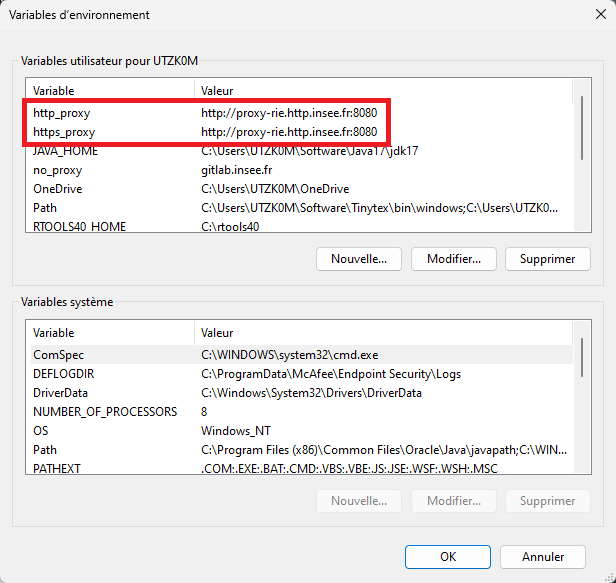
\includegraphics{../img/modify_proxy.png}

\hypertarget{java_home-1}{%
\subsubsection{JAVA\_HOME}\label{java_home-1}}

De même pour la variable d'environnement \texttt{JAVA\_HOME} pour
Windows, comme pour la configuration du proxy, il faut :

\begin{itemize}
\tightlist
\item
  Rechercher ``Modifier les variables d'environnement pour votre
  compte''
\item
  Cliquer sur l'application
\item
  Ajouter une variable \texttt{JAVA\_HOME} si elle n'existe pas et la
  modifier si elle existe :
\end{itemize}

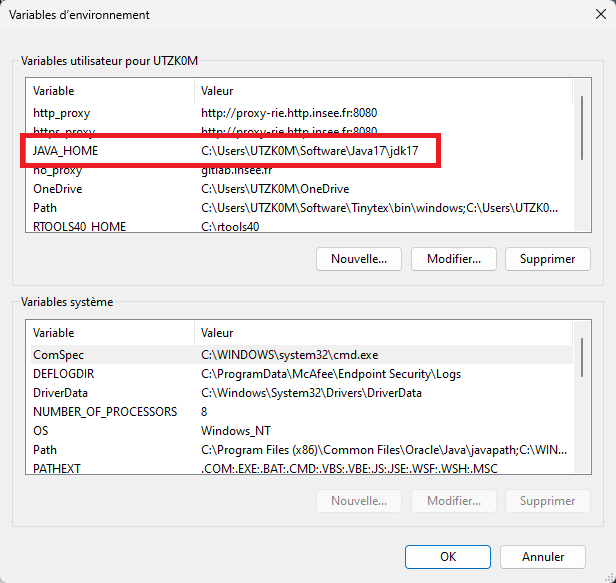
\includegraphics{../img/modify_java_home.png}

\hypertarget{path}{%
\subsubsection{PATH}\label{path}}

La variable d'environnement \texttt{PATH} en \textbf{R} sert à indiquer
à \textbf{R} où chercher les fichiers exécutables.

Lorsque vous installer un nouveau logiciel \emph{(exemple JDemetra+,
Rtools, Java\ldots)} dont Rstudio fera appel, il faut modifier cette
variable d'environnement :

\begin{itemize}
\item
  \textbf{Récupérer} l'actuelle valeur de la variable \texttt{PATH} via
  la commande
  \VERB|\FunctionTok{Sys.getenv}\NormalTok{(}\StringTok{"PATH"}\NormalTok{)}|
  (Rstudio renvoie alors une succession d'adresse du type
  \texttt{C:/WINDOWS/system32;C:/WINDOWS})
\item
  \textbf{Copier-coller} ces adresses après \texttt{PATH\ =} et y
  ajouter les chemins vers les répertoires
  \textcolor{windows_path_color}{\nolinkurl{\\bin\\}} (binary) des
  logiciels nouvellement installés, en les séparant par des
  points-virgules sans espace avant ni après.

  Par exemple, pour l'installation de Rtools, le chemin est
  \textcolor{windows_path_color}{\nolinkurl{C:\\rtools42\\mingw64\\bin}}
  (selon là où a été installé Rtools). Il faut donc rajouter
  \texttt{C:\textbackslash{}\textbackslash{}rtools42\textbackslash{}\textbackslash{}mingw64\textbackslash{}\textbackslash{}bin}
  ou \texttt{C:/rtools42/mingw64/bin} (En \textbf{R},
  \texttt{\textbackslash{}} est un caractère spécial, donc il faut
  remplacer les \texttt{\textbackslash{}} par \texttt{/} ou par
  \texttt{\textbackslash{}\textbackslash{}}). Le chemin devient
  \texttt{C:/WINDOWS/system32;C:/WINDOWS;C:/rtools42/mingw64/bin}.
\item
  \textbf{Modifier} la variable avec la fonction
  \VERB|\FunctionTok{Sys.setenv}\NormalTok{()}|.

  Pour l'exemple ci-dessus, la commande à lancer est :

\begin{Shaded}
\begin{Highlighting}[]
\FunctionTok{Sys.setenv}\NormalTok{(}\AttributeTok{PATH =} \StringTok{"C:/WINDOWS/system32;C:/WINDOWS;C:/rtools42/mingw64/bin"}\NormalTok{)}
\end{Highlighting}
\end{Shaded}
\end{itemize}

ℹ️ NB : Généralement une version 32 bits et une version 64 bits sont
disponibles au téléchargement et à l'installation d'un logiciel. Il faut
vérifier le type de processeur de votre Système d'exploitation afin de
choisir le bon dossier propre à votre version système.

Pour cela, vous pouvez lancer les commandes suivantes :

\begin{Shaded}
\begin{Highlighting}[]
\FunctionTok{Sys.getenv}\NormalTok{(}\StringTok{"R\_ARCH"}\NormalTok{)}
\FunctionTok{Sys.info}\NormalTok{()[[}\StringTok{"machine"}\NormalTok{]]}
\end{Highlighting}
\end{Shaded}

Selon le résultat, la version est 32 bits ou 64 bits :

\begin{longtable}[]{@{}
  >{\raggedright\arraybackslash}p{(\columnwidth - 2\tabcolsep) * \real{0.1806}}
  >{\raggedright\arraybackslash}p{(\columnwidth - 2\tabcolsep) * \real{0.1944}}@{}}
\toprule()
\begin{minipage}[b]{\linewidth}\raggedright
Version
\end{minipage} & \begin{minipage}[b]{\linewidth}\raggedright
Output
\end{minipage} \\
\midrule()
\endhead
\multirow{2}{*}{64 bits} & /x64 \\
& x86-64 \\
& \\
\multirow{2}{*}{32 bits} & /i386 \\
& x86\_32 \\
\bottomrule()
\end{longtable}

Plus d'informations sur la variable \texttt{PATH} via la page
\textcolor{html_color}{\url{https://java.com/fr/download/help/path.xml}}.

\hypertarget{vuxe9rifications}{%
\section{Vérifications}\label{vuxe9rifications}}

Pour s'assurer que tout fonctionne bien, on peut faire tourner des
exemples de code et vérifier qu'il n'y a pas d'erreurs :

\begin{Shaded}
\begin{Highlighting}[]
\FunctionTok{library}\NormalTok{(}\StringTok{"RJDemetra"}\NormalTok{)}

\NormalTok{myseries }\OtherTok{\textless{}{-}}\NormalTok{ ipi\_c\_eu[, }\StringTok{"FR"}\NormalTok{]}
\NormalTok{x13\_model }\OtherTok{\textless{}{-}} \FunctionTok{x13}\NormalTok{(myseries) }\CommentTok{\# X{-}13ARIMA method}
\NormalTok{ts\_model }\OtherTok{\textless{}{-}} \FunctionTok{tramoseats}\NormalTok{(myseries) }\CommentTok{\# TRAMO{-}SEATS method}

\CommentTok{\# Basic plot with the original series, the trend and the SA series}
\FunctionTok{plot}\NormalTok{(x13\_model, }\AttributeTok{type\_chart =} \StringTok{"sa{-}trend"}\NormalTok{)}
\end{Highlighting}
\end{Shaded}

Pour vérifier la version de Java que l'on utilise sous \textbf{R}, on
peut essayer d'installer et utiliser le package \textbf{rJava} et lancer
la commande ci-dessous :

\begin{Shaded}
\begin{Highlighting}[]
\CommentTok{\# Si le package rJava n\textquotesingle{}est pas installé}
\FunctionTok{install.packages}\NormalTok{(}\StringTok{"rJava"}\NormalTok{)}
\end{Highlighting}
\end{Shaded}

Si l'installation de \textbf{rJava} retourne une erreur, cela veut dire
que Java a été mal installé ou mal configuré sur \textbf{R}. Il faut
retourner à la section \protect\hyperlink{var_env}{Variables
d'environnement}.

Ce bloc de commande teste la version de Java avec laquelle \textbf{R}
fonctionne :

\begin{Shaded}
\begin{Highlighting}[]
\FunctionTok{library}\NormalTok{(}\StringTok{"rJava"}\NormalTok{)}
\FunctionTok{.jinit}\NormalTok{()}
\FunctionTok{.jcall}\NormalTok{(}\StringTok{"java/lang/System"}\NormalTok{, }\StringTok{"S"}\NormalTok{, }\StringTok{"getProperty"}\NormalTok{, }\StringTok{"java.runtime.version"}\NormalTok{)}
\end{Highlighting}
\end{Shaded}

Enfin, on peut consulter la version de Java installé sur notre poste et
avec laquelle Windows fonctionne (cela n'a pas d'importance pour nous) :

\begin{Shaded}
\begin{Highlighting}[]
\FunctionTok{system}\NormalTok{(}\StringTok{"java {-}version"}\NormalTok{)}
\end{Highlighting}
\end{Shaded}

\hypertarget{installations-optionnelles}{%
\section{Installations optionnelles}\label{installations-optionnelles}}

Certaines installations supplémentaires sont optionnelles (c'est-à-dire
qu'elles ne sont pas obligatoires mais apportent des fonctionnalités
externes) :

\begin{itemize}
\tightlist
\item
  \href{https://miktex.org/howto/install-miktex}{Miktek} pour produire
  des documents latex
\item
  \href{https://cran.r-project.org/bin/windows/Rtools/rtools42/rtools.html}{Rtools}
  pour développer des packages et compiler du code
\end{itemize}

\hypertarget{probluxe8mes-que-lon-peut-rencontrer}{%
\section{Problèmes que l'on peut
rencontrer}\label{probluxe8mes-que-lon-peut-rencontrer}}

\hypertarget{probluxe8me-dinstallation-de-package-r}{%
\subsection{\texorpdfstring{Problème d'installation de package
\textbf{R}}{Problème d'installation de package R}}\label{probluxe8me-dinstallation-de-package-r}}

Si lors de l'installation de packages, vous obtenez l'erreur suivante :

\begin{Shaded}
\begin{Highlighting}[]
\FunctionTok{install.packages}\NormalTok{(}\StringTok{"RJDemetra"}\NormalTok{)}
\end{Highlighting}
\end{Shaded}

\begin{verbatim}
## Error in eval(expr, envir, enclos): Erreur : le chargement a échoué
## Exécution arrêtée
## *** arch - x64
\end{verbatim}

Le problème ne vient pas de Java mais du package \textbf{R}. Par défaut,
le package s'installe depuis le fichier ``source'', c'est-à-dire que le
package est recompilé. Pour certaines raisons informatiques, lorsqu'on
compile par défaut, ce sont les paramètres système de base qui sont
utilisés (et qui n'ont pas forcément les bonnes versions de Java).

Deux solutions :

\begin{itemize}
\item
  Compiler le package en installant depuis le ``binary'' :

\begin{Shaded}
\begin{Highlighting}[]
\FunctionTok{install.packages}\NormalTok{(}\StringTok{"RJDemetra"}\NormalTok{, }\AttributeTok{type =} \StringTok{"binary"}\NormalTok{)}
\end{Highlighting}
\end{Shaded}
\item
  Spécifier que l'on veut utiliser les paramètres locaux :

\begin{Shaded}
\begin{Highlighting}[]
\FunctionTok{install.packages}\NormalTok{(}\StringTok{"RJDemetra"}\NormalTok{, }\AttributeTok{type =} \StringTok{"source"}\NormalTok{, }\AttributeTok{INSTALL\_opts =} \StringTok{"{-}{-}no{-}multiarch"}\NormalTok{)}
\end{Highlighting}
\end{Shaded}
\end{itemize}

ℹ️ Plus d'information :
\textcolor{html_color}{\url{https://github.com/jdemetra/rjdemetra/wiki/Installation-manual}}

\hypertarget{la-commande-libraryrjdemetra-renvoie-un-message-derreur}{%
\subsection{\texorpdfstring{La commande \texttt{library("RJDemetra")}
renvoie un message
d'erreur}{La commande library("RJDemetra") renvoie un message d'erreur}}\label{la-commande-libraryrjdemetra-renvoie-un-message-derreur}}

Le package {\textbf{\{RJDemetra\}}} a besoin de la version 8 (au
minimum) de Java pour fonctionner. Si au moins un autre package a déjà
été chargé via la fonction \VERB|\FunctionTok{library}\NormalTok{()}| et
qu'il ne nécessite pas une version très à jour de Java, c'est cette
ancienne version qui sera sollicitée pendant toute la durée de la
session (\textbf{R} est réfractaire au changement de version en cours de
session). En cas d'utilisation de {RJDemetra} au cours d'un programme,
il faut donc impérativement spécifier dès le début de programme que
\textbf{R} aille chercher la version 8, via la commande :

\begin{Shaded}
\begin{Highlighting}[]
\CommentTok{\# Là où est installé java}
\FunctionTok{Sys.setenv}\NormalTok{(}\AttributeTok{JAVA\_HOME =} \StringTok{"C:/Users/Software/Java17/jdk17"}\NormalTok{)}
\end{Highlighting}
\end{Shaded}

ou charger {\textbf{\{RJDemetra\}}} en premier

\begin{Shaded}
\begin{Highlighting}[]
\CommentTok{\# En début de programme}
\FunctionTok{library}\NormalTok{(}\StringTok{"RJDemetra"}\NormalTok{)}
\end{Highlighting}
\end{Shaded}

Sinon il faut redémarrer une nouvelle session \textbf{R}.

\hypertarget{error-array-index--1}{%
\subsection{\texorpdfstring{\texttt{Error\ array\ index\ =\ -1}}{Error array index = -1}}\label{error-array-index--1}}

Le message du type \texttt{Error\ array\ index\ =\ -1} indique une
variable auxiliaire non trouvée. Il peut s'agir de régresseurs CJO ou
d'autres variables définies par l'utilisateur (effet de Pâques
spécifique, PSO = pure seasonal outlier\ldots).

\hypertarget{la-fonction-cruncher_and_param...-du-package-jdcruncher-renvoie-un-message-derreur}{%
\subsection{\texorpdfstring{La fonction
\texttt{cruncher\_and\_param(...)} du package {\textbf{\{JDCruncheR\}}}
renvoie un message
d'erreur}{La fonction cruncher\_and\_param(...) du package \{JDCruncheR\} renvoie un message d'erreur}}\label{la-fonction-cruncher_and_param...-du-package-jdcruncher-renvoie-un-message-derreur}}

Lorsqu'on lance la fonction
\VERB|\FunctionTok{cruncher\_and\_param}\NormalTok{(...)}| du package
{\textbf{\{JDCruncheR\}}}, on peut obtenir l'erreur suivante :

\begin{verbatim}
## Error in eval(expr, envir, enclos): Error in cruncher(workspace = workspace, cruncher_bin_directory = cruncher_bin_directory,  : 
##   There is an error in the path to the cruncher bin folder
\end{verbatim}

Cela veut dire que le chemin jusqu'au cruncher a mal été configuré. Pour
remédier à cela, il faut préciser à R le chemin du cruncher en début de
programme avec la fonction \VERB|\FunctionTok{options}\NormalTok{(...)}|
:

\begin{Shaded}
\begin{Highlighting}[]
\FunctionTok{options}\NormalTok{(}\AttributeTok{cruncher\_bin\_directory =} \StringTok{"C:/Users/Software/jwsacruncher{-}2.2.4{-}bin/bin"}\NormalTok{)}
\end{Highlighting}
\end{Shaded}

Pour vérifier que le chemin est bien valide, il faut utiliser la
fonction \VERB|\FunctionTok{getOption}\NormalTok{(...)}| :

\begin{Shaded}
\begin{Highlighting}[]
\FunctionTok{getOption}\NormalTok{(}\StringTok{"cruncher\_bin\_directory"}\NormalTok{)}
\end{Highlighting}
\end{Shaded}


\end{document}
